%====================================================
%
% Author: Dipl.-Inf. Xavier NOUMBISSI NOUNDOU, Ph.D.-Candidate
% Email:  xnoundou7@gmail.com
%
%====================================================
\documentclass[10pt, a4paper]{bookest}
\NeedsTeXFormat{LaTeX2e}
\makeindex

%---------------------------- PACKAGE INCLUSION -------------------------------
% This group renders characters clearer and more precise

\RequirePackage[bitstream-charter,cal,expert]{mathdesign}
\RequirePackage{makeidx}
\RequirePackage{latexsym}

\usepackage{geometry} % to change the page dimensions
\geometry{a4paper,
		  %showframe=true,
		  %margin=3cm,
		  %a4paper,
		  %total={170mm,257mm},
		  top=4.15em,
		  left=5.5em,
		  right=5.5em,
		  bottom=3.39em
		  }

\usepackage[default]{cantarell}
\usepackage{graphicx}
\usepackage[french]{babel}
\usepackage{xspace}
\usepackage[parfill]{parskip} % Activate to begin paragraphs with an empty line rather than an indent
\usepackage{paralist} % very flexible & customisable lists (eg. enumerate/itemize, etc.)
\usepackage{listings} % for lstset definitions
\usepackage{url}
\usepackage{subfig} % make it possible to include more than one captioned figure/table in a single float
\usepackage{epsfig}
\usepackage{booktabs}
%\usepackage{enumitem} %funny itemize icons
\usepackage{verbatim}

\usepackage{amsmath}
\newcommand{\mathbold}[1]{\text{\textbf{#1}}}

\usepackage{xcolor}
\definecolor{forestgreen}{RGB}{2,160,70}    
\definecolor{mediumblue}{RGB}{7,43,205}    
\definecolor{firebrickred}{RGB}{178,34,34}
\definecolor{listingray}{gray}{0.9}
\definecolor{lbcolor}{rgb}{0.9,0.9,0.9}
\definecolor{darkgreen}{rgb}{0,0.35,0}
\definecolor{medgreen}{rgb}{0,0.5,0}
\definecolor{lightgreen}{rgb}{0.5,0.7,0.5}
\definecolor{pmcolour}{rgb}{0.5,0.7,0.5}
\definecolor{medgrey}{rgb}{0.6,0.6,0.6}
\definecolor{purplish}{rgb}{0.4,0,0.6}
\definecolor{brightred}{rgb}{1,0.2,0.2}

\newcommand{\diplominformatiker}{Diplom--Informatiker\xspace}

\newcommand{\diplinfn}{Dipl.--Inf.\xspace}

\newcommand{\pos}{syst\`eme--logiciel ERP\xspace}

\newcommand{\yerenlabs}{\textsc{Yeroth-R\&D}\xspace}

\newcommand{\yerenpos}{\textcolor{yerenColorBlue}{\sc YEROTH--ERP--$3.0$}\xspace}

\newcommand{\myfullacademicname}{Xavier NOUMBISSI NOUNDOU, Ph.D. (ABD)\xspace}

\usepackage{hyperref}
\hypersetup{
    colorlinks,
	pagebackref,
    citecolor=medgreen,
    linkcolor=purplish,
    breaklinks,
    pdftex,
    bookmarks,
    plainpages=false,
	pdftitle={Manuel de l'Utilisateur ''Gestionaire de Stocks'' de YEROTH--ERP (version $3.0$)
				par \myfullacademicname},
    pdfauthor={Xavier NOUMBISSI NOUNDOU, Ph.D. (ABD)}
}

%--------------------------------------------------------------------------------

%---------------------------- COMMANDS DEFINITION -------------------------------
\newcommand{\tool}[1]{\texttt{\textbf{#1}}\xspace}
\newcommand{\UUT}{Unit Under Test\xspace}
\newcommand{\annotation}[1]{ \texttt{\textbf{#1}}\xspace}
\newcommand{\junit}{\texttt{\textbf{JUnit}}\xspace}
\newcommand{\company}[1]{\textbf{#1}\xspace}
\newcommand{\diplinf}{\textsc{Dipl.-Inf.}\xspace}
\newcommand{\saint}{\textbf{\textsc{SAINT}}\xspace}

\newcommand{\emphbf}[1]{\textbf{#1}\xspace}
\newcommand{\emphit}[1]{\emph{\textit{#1}}\xspace}
\newcommand{\mycheckmark}[1]{\textcolor{#1}{$\checkmark$}\xspace}
\newcommand{\mytimes}[1]{\textcolor{#1}{$\times$}\xspace}
\newcommand{\boldsc}[1]{\textbf{\textsc{#1}}\xspace}

\newcommand{\myenumitem}[1]{\emph{#1}\xspace}

\newcommand{\bergmann}{Bergmann Automaten GmbH\xspace}
\newcommand{\siemens}{\textsc{Siemens} Medical Solutions\xspace}
\newcommand{\watformlab}{Watform Lab\xspace}
\newcommand{\uwaterloo}{University of Waterloo\xspace}


\newcommand{\javalanguage}{\emph{Java}\xspace}
\newcommand{\vmodel}{\emph{V-Model}\xspace}

\newcommand{\yeren}{\textsc{yeroth--erp--3.0}\xspace}
\newcommand{\yerenalert}{\emph{yeroth--erp--alert--3.0}\xspace}
\newcommand{\mysql}{MySQL\xspace}
\newcommand{\depot}{d\'ep\^ot\xspace}
\newcommand{\depots}{d\'ep\^ots\xspace}
\newcommand{\bouton}[1]{"\textbf{#1}"\xspace}
\newcommand{\field}[1]{"\emph{\textbf{#1}}"\xspace}

\newcommand{\role}{r\^ole\xspace}
\newcommand{\roles}{r\^oles\xspace}
\newcommand{\manager}{\emph{Manager}\xspace}
\newcommand{\gestionairedestocks}{\emph{GestionaireDeStocks}\xspace}
\newcommand{\magasinier}{\emph{Magasinier}\xspace}
\newcommand{\caissier}{\emph{Caissier}\xspace}
\newcommand{\admin}{\emph{Administrateur}\xspace}

\newcommand{\qt}{Qt$5.7$\xspace}

\newcommand{\managerb}{\emph{\textbf{Manager}}\xspace}
\newcommand{\gestionairedestocksb}{\emph{\textbf{GestionaireDeStocks}}\xspace}
\newcommand{\caissierb}{\emph{\textbf{Caissier}}\xspace}
\newcommand{\administrateurb}{\emph{\textbf{Administrateur}}\xspace}
\newcommand{\magasinierb}{\emph{\textbf{Magasinier}}\xspace}

\newcommand{\utilisateurs}
	{\textcolor{blue}{\textbf{\emph{R\^oles ayant acc\`es \`a la fonctionalit\'e}}}\xspace}
	
\newcommand{\optionel}{\textcolor{firebrickred}{\textbf{\emph{[optionel]}}}\xspace}

\newcommand{\lienmagasinier}{\magasinier~\ref{sec:utilisateurs-lemagasinier}\xspace}
\newcommand{\liencaissier}{\caissier~\ref{sec:utilisateurs-lecaissier}\xspace}
\newcommand{\lienadmin}{\admin~\ref{sec:utilisateurs-ladministrateur}\xspace}
\newcommand{\lienmanager}{\manager~\ref{sec:utilisateurs-lepatron}\xspace}
\newcommand{\yerenfield}[1]{\textbf{\emph{#1}}\xspace}
\newcommand{\procparagraph}[1]
	{\paragraph{ \mycheckmark{forestgreen} \emph{\textcolor{forestgreen}{#1}}}}

\newcommand{\xavier}{Xavier NOUMBISSI NOUNDOU\xspace}

\newcommand{\reference}{r\'ef\'erence\xspace}

\newcommand{\cmup}{\textbf{CMUP}\xspace}
\newcommand{\dpfdpo}{\textbf{DEF\_DEO}\xspace}
\newcommand{\fifo}{\textbf{FIFO}\xspace}
\newcommand{\lifo}{\textbf{LIFO}\xspace}

\newcommand{\fenetre}{fen\^etre\xspace}
\newcommand{\uielemone}[1]{\textcolor{medgreen}{\emph{#1}}\xspace}
\newcommand{\uielemtwo}[1]{\textcolor{mediumblue}{\texttt{#1}}\xspace}

\newcommand{\nxsection}[1]{\section{#1}\xspace}
\newcommand{\nxsubsection}[1]{\subsection{#1}\xspace}
\newcommand{\chapintro}[1]{\textcolor{purplish}{\emph{#1}}\xspace}

%\usepackage{makeidx} % Used to generate the index
%\makeindex % Generate the index which is printed at the end of the document

%--------------------------------------------------------------------------------

\usepackage[T1]{fontenc}
\newcommand{\changefont}[3]{
\fontfamily{#1} \fontseries{#2} \fontshape{#3} \selectfont}
\changefont{cmss}{m}{n}

% Set font to avant-garde
%\renewcommand*\rmdefault{pag}

%Remove widows and orphants
\clubpenalty = 10000
\widowpenalty = 10000
\displaywidowpenalty = 10000

\begin{document}
\frontmatter\pagestyle{plain}
\title{\textcolor{medgreen}{\textsc{Syst\`eme--Logiciel ERP
		\\ \vspace*{1.5cm}(\yeren)\\}
		\vspace*{3cm}
	Manuel de l'Utilisateur\\ \vspace{1em} << Gestionaire de Stocks >>}}

\begin{titlepage}
\maketitle
\vspace{\stretch{2}}
\centering
\copyright\ \textsc{\myfullacademicname}
\end{titlepage}

% TABLE OF CONTENTS
\cleardoublepage
\phantomsection
\addcontentsline{toc}{chapter}{\contentsname}
\begingroup
\color{medgreen}
\tableofcontents
\endgroup

% LIST OF TABLES
\cleardoublepage
\phantomsection
\addcontentsline{toc}{chapter}{\listtablename}
\begingroup
\color{medgreen}
\listoftables
\endgroup

% LIST OF FIGURES
\cleardoublepage
\phantomsection
\addcontentsline{toc}{chapter}{\listfigurename}
\begingroup
\color{medgreen}
\listoffigures
\endgroup

\cleardoublepage
\phantomsection
\addcontentsline{toc}{chapter}{\`A propos de l'auteur}
\chapter*{\`A propos de l'auteur}\label{chap:biography}
\index{\`a propos de l'auteur}
\index{biographie de l'auteur}

\begin{figure}[!htpb]
\centering
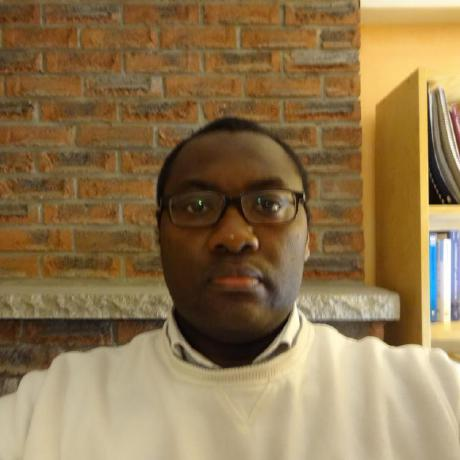
\includegraphics[scale=0.63]{images/XavierNOUNDOU-2}
\caption{Portrait de Xavier}~\label{fig:xaviernoumbis}
\end{figure}


\mainmatter

\chapter{Introduction}\label{chap:introduction}

\yeren est un syst\`eme logiciel de gestion des
stocks et de gestion des ventes. Il permet
d'ex\'ecuter des mouvements de stocks, et de
vendre des articles en stocks.

Une entreprise doit poss\'eder au minimum d'un stock
d'articles, d'un d\'ep\^ot ou d'une boutique pour utiliser
\yeren de fa\c{c}on efficace.\\

\begin{figure}[!htpb]
	\centering
	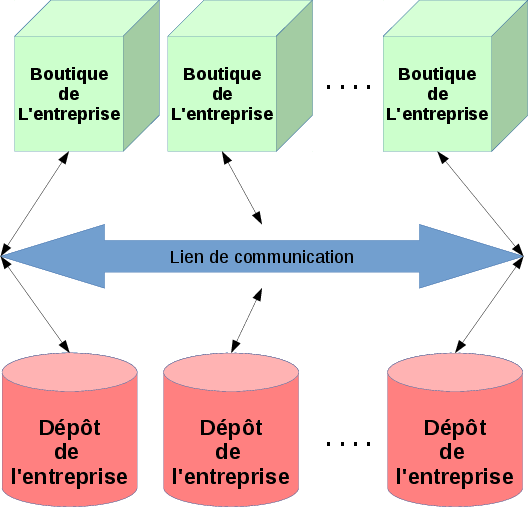
\includegraphics[scale=0.63]{images/architecture-enterprise-yeren.png}
	\caption{Un mod\`ele d'architecture d'une entreprise}\label{fig:architecture-enterprise-yeren}
\end{figure}

La figure~\ref{fig:architecture-enterprise-yeren} illustre
un mod\`ele g\'en\'erique d'entreprise o\`u les d\'ep\^ots
et les boutiques de l'entreprise sont en communication.

Les activit\'es principales de l'entreprise sont les suivantes:
\begin{enumerate}[1)]
	\item \emphbf{les sorties de stocks:} sortie d'articles
		d'une unit\'e (boutique ou d\'ep\^ot) pour r\'eception par un client
	\item \emphbf{les transferts de stocks:} mouvement d'articles
		d'une unit\'e vers une autre unit\'e
	\item \emphbf{les ventes d'articles:} un client ach\`ete
		des articles qui lui sont ensuite remis.\\
\end{enumerate}

\yeren permet d'accomplir les t\^aches de gestion
des stocks et de gestion des ventes suivantes:
\begin{enumerate}[1)]
	\item \myenumitem{cr\'eer des alertes sur des p\'eriodes de temps}	
	\item \myenumitem{cr\'eer des alertes sur des quantit\'e en stocks}	
	\item \myenumitem{entrer un stock}
	\item \myenumitem{lister les stocks}
	\item \myenumitem{modifier un stock}
	\item \myenumitem{supprimer un stock}	
	\item \myenumitem{rechercher des articles ou des stocks}
	\item \myenumitem{transf\'erer des articles ou des stocks}	
	\item \myenumitem{vendre des articles}	
	\item \myenumitem{visualiser les \'etats de transactions d'articles
		(sorties ou transferts de stocks)}
	\item \myenumitem{acc\'eder aux tableaux de bords}
	\item \myenumitem{visualiser les \'etats de ventes d'articles}.\\
\end{enumerate}

\newpage

\section{Acc\`es au manuel de l'utilisateur}

La figure~\ref{fig:fenetre-principale-utilisateur-non-enregistre}
illustre la fen\^etre d'accueil de \yeren sans aucun utilisateur
enregistr\'e.\\

\begin{figure}[!htbp]
\centering
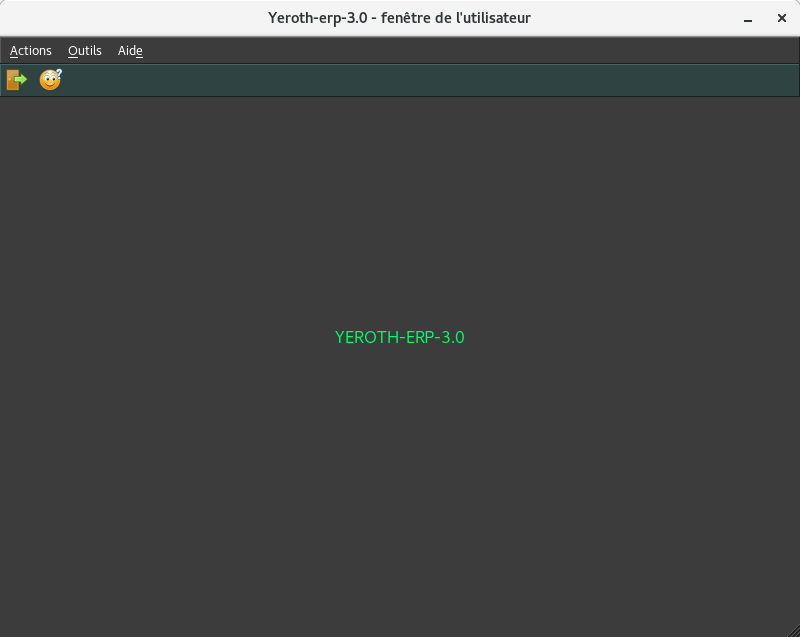
\includegraphics[scale=0.63]{images/yeren-fenetre-principale.png}
\caption{La fen\^etre d'acceuil sans aucun utilisateur enregistr\'e.}
\label{fig:fenetre-principale-utilisateur-non-enregistre}
\end{figure}

Il est requis qu'un utilisateur soit enregistr\'e
dans \yeren afin d'avoir acc\`es au manuel de l'utilisateur.

L'utilisateur de \yeren doit accomplir les op\'erations
suivantes afin d'avoir acc\`es au manuel de l'utilisateur:
\begin{enumerate}[1)]
	\item \`a partir de la fen\^etre d'accueil
		(voir figure~\ref{fig:fenetre-principale-utilisateur-non-enregistre}),
		cliquez sur le menu d\'eroulant '\textbf{Aide}'
	\item ensuite cliquez sur le lien '\textbf{Manuel de l'utilisateur (PDF)}'.
\end{enumerate}

\section{Structure de ce manuel de l'utilisateur}
Ce manuel de  l'utilisateur de \yeren est structur\'e
comme suit:

\begin{itemize}[\mycheckmark{purplish}]
	\item le chapitre~\ref{chap:utilisateurs} d\'ecrit
	les utilisateurs de \yeren et leurs \roles. 
	     
	\item le chapitre~\ref{chap:gestion-stocks} explicite
	les fonctionalit\'es de gestion des stocks

	\item le chapitre~\ref{chap:gestion-des-achats} parle
	de la gestion des achats
	
	\item le chapitre~\ref{chap:systeme-dalertes}
	pr\'esente le syst\`eme d'alertes sur les stocks
	
	\item le chapitre~\ref{chap:vendre} d\'ecrit comment
	conclure des ventes d'articles
	
	\item le chapitre~\ref{chap:sortir-articles} d\'ecrit
	comment proc\'eder \`a des sorties et transferts de stocks
	
	\item le chapitre~\ref{chap:vente} explicite comment
	rechercher et imprimer les \'etats de ventes d'articles
	
	\item le chapitre~\ref{chap:etats-des-sorties} explicite
	comment rechercher et imprimer les \'etats de sorties ou
	transferts d'articles
	
	\item le chapitre~\ref{chap:tableaux-de-bord} discute
	de la recherche et de la g\'en\'eration des rapports
	commerciaux de l'entreprise
	
	\item le chapitre~\ref{chap:informations-generales}
	explique comment avoir acc\`es aux d\'etails de
	l'utilisateur enregistr\'e, aux informations commerciales
	de l'entreprise, et enfin \`a la version de \yeren que
	l'on utilise
	
	\item le chapitre~\ref{chap:administration-logiciel}
	traite de l'administration du logiciel

	\item le chapitre~\ref{chap:problemes-connues}
	discute des probl\`emes connues de \yeren
	
	\item enfin, le chapitre~\ref{chap:conclusion} conclut
	ce manuel d'utilisation.
\end{itemize}


\nxsection{Le r\^ole ''GestionaireDeStocks''}\label{sec:utilisateurs-gestionairedestocks}
\index{gestionaire de stocks}
\index{GestionaireDeStocks}

La figure~\ref{fig:yeren-fenetre-gestionairedestocks} illustre
la fen\^etre d'acceuil d'un utilisateur avec le \role \gestionairedestocks, 
apr\`es qu'il se soit enregistr\'e dans \yeren.\\

\begin{figure}[!htbp]
\centering
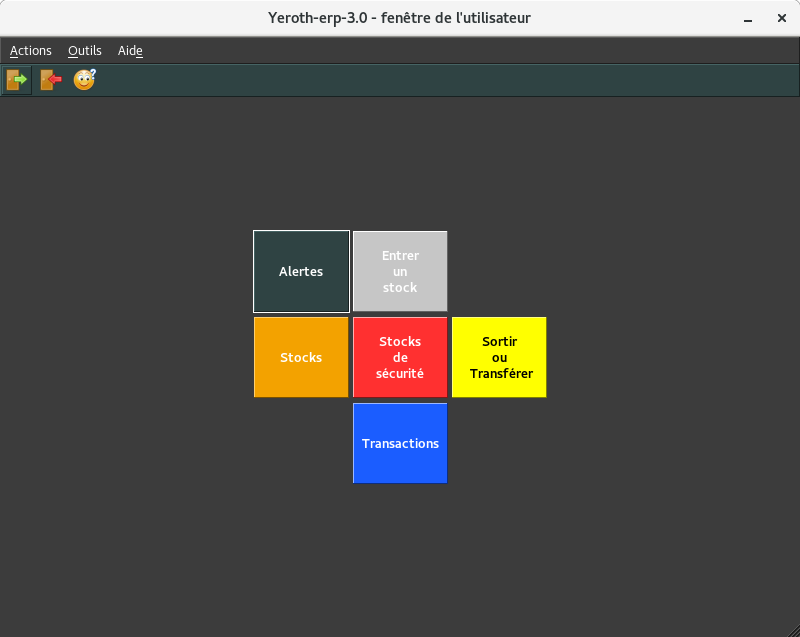
\includegraphics[scale=0.63]{images/yeren-fenetre-gestionairedestocks.png}
\caption{La fen\^etre d'acceuil d'un gestionaire de stocks}
\label{fig:yeren-fenetre-gestionairedestocks}
\end{figure}
\chapter{La Gestion des Stocks}\label{chap:gestion-stocks}
\index{la gestion des stocks}

\utilisateurs: \lienmagasinier.\\

\chapintro{Ce chapitre d\'ecrit comment avoir acc\`es aux
fonctionalit\'es de gestion des stocks et comment les utiliser.}

\nxsection{Introduction}

Les t\^aches de gestion des stocks sont illustr\'ees
dans le Tableau~\ref{tab:taches-fonctions}, en fonction
du r\^ole de l'utilisateur.\\

\begin{table}[!htbp]
\centering
\begin{tabular}{lccccc}
\textbf{T\^aches} 							& \managerb		 & \vendeurb	 		&	\gestionairedestocksb	& \magasinierb		& \caissierb 		\\ \hline
entrer un stock 							& \mycheckmark{blue} & 				 		& \mycheckmark{blue}			& 					&  				 	\\ \hline
supprimer un stock 							& \mycheckmark{blue} & 				 		& 							&					&  					\\ \hline
lister les marchandises 					& \mycheckmark{blue} &\mycheckmark{blue} 		& \mycheckmark{blue} & 	& \\ \hline
lister les stocks 							& \mycheckmark{blue} &\mycheckmark{blue} 		& \mycheckmark{blue}			& \mycheckmark{blue}	& \mycheckmark{blue} 	\\ \hline
modifier un stock 							& \mycheckmark{blue} & 				 		& \mycheckmark{blue}			& 					&  				 	\\ \hline
transf\'erer des stocks 					& \mycheckmark{blue} & 				 		& \mycheckmark{blue}			& \mycheckmark{blue}	&  				 	\\ \hline
sortir des stocks							& \mycheckmark{blue} & 				 		& \mycheckmark{blue}			& \mycheckmark{blue}	&  				 	\\ \hline
modifier la strat\'egie 					&  				 & 				 		& 							& 					&	 				\\ 
de gestion des stocks  						& \mycheckmark{blue} & \mytimespartial{blue}& \mytimespartial{blue}		& 					&  				 	\\ 
(ex.: \fifo, etc.)							&				 &				 		&							&					&					\\ \hline
vendre des marchandises 					& \mycheckmark{blue} & \mycheckmark{blue} 		&				 			& 					& \mycheckmark{blue} 	\\ \hline
acc\'eder aux  		 						& 				 &				 		&				 			& 					&  				 	\\ 
mouvements des stocks 	   		 			& \mycheckmark{blue} & 				 		&\mycheckmark{blue}				& \mycheckmark{blue}  	&				 	\\
\end{tabular}
\caption{Tableau des t\^aches et des r\^oles associ\'es
\`a la gestion des stocks}
\label{tab:taches-fonctions}
\index{t\^aches de gestion des stocks}
\end{table}

\nxsection{Les strat\'egies de gestion des stocks}\label{sec:strategies-gestion-stocks}
\index{strat\'egies de gestion des stocks}
\index{strat\'egie de sortie des articles}
\index{strat\'egie de vente des articles}
\index{strat\'egie de gestion des stocks ! \cmup}
\index{strat\'egie de gestion des stocks ! \dpfdpo}
\index{strat\'egie de gestion des stocks ! \fifo}
\index{strat\'egie de gestion des stocks ! \lifo}

\yeren impl\'emente $4$ strat\'egies pour g\'erer les stocks \`a
vendre ou \`a sortir:
\begin{enumerate}[1)]
	\item \cmup: Cours Moyen, Unit\'e Pond\'er\'ee.
	
		La strat\'egie \cmup affiche tous les 
		stocks de \facon (Cours
		Moyen, Unit\'e Pond\'er\'ee).\\
		
	\item \dpfdpo: Date of Expiration First, Date of Expiration Out.
	
		La strat\'egie \dpfdpo affiche les
		stocks \`a vendre ou \`a sortir selon
		le principe: les stocks avec des dates
		de p\'eremption les plus proches sont 
		les premiers \`a sortir.\\
		
	\item \fifo: First In, First Out. 
	
		La strat\'egie \fifo affiche les stocks
		\`a vendre ou \`a sortir selon le principe
		''\textbf{First In, First Out}'':
		Les stocks avec des dates d'entr\'ee en stock
		plus anciennes sont les premiers \`a sortir.\\
		
	\item \lifo: Last In, First Out.
	
		La strat\'egie \lifo affiche les stocks
		\`a vendre ou \`a sortir selon le principe
		''\textbf{Last In, First Out}'': 
		Les stocks avec des dates d'entr\'ee en stock
		plus r\'ecentes sont les premiers \`a sortir.\\
\end{enumerate}
\index{\cmup}
\index{\dpfdpo}
\index{\fifo}
\index{\lifo}

La strat\'egie de gestion des stocks se modifie
comme suit:

\begin{itemize}[\mycheckmark{purplish}]
	\item de \facon permanente dans
		la section 'administration' de \yerenpos.

	\item de \facon temporaire (\`a des fins de
		visualitation de l'ordre des sorties de
		stocks) dans la \fenetre 
		\textbf{'fiche des stocks'} de \yerenpos.
\end{itemize}

%\newpage

%-----------------------------------------------------------

\nxsection{Entrer un stock}
\index{entrer un stock}
\index{stock minimum}

\yeren entretient les donn\'ees suivantes pour chaque stock:
\begin{enumerate}[1)]
	\item la cat\'egorie \obligatoire
	\item la d\'esignation \obligatoire
	\item la date de p\'eremption du stock 
	\item le fournisseur 
	\item la localisation du stock
	\item le montant de la TVA d'un article 
	\item le prix de vente d'un article \obligatoire
	\item la quantit\'e intiale (nombre de lots, et quantit\'e par lot) \obligatoire
	\item la \reference
	\item la \reference du re\c{c}u d'achat
	\item le stock minimum: si cette quantit\'e
		est atteinte, alors le nombre de la colone 'Qt\'e totale'
		du stock est affich\'e en rouge.\\
\end{enumerate}

Il existe deux m\'ethodes pour entrer un stock dans \yeren:
\begin{enumerate}[1)]
	\item la $\mathbf{1^{\textbf{\`ere}}}$ \textbf{m\'ethode}
	est utilis\'ee pour entrer un stock d'articles \`a partir
	d'un formulaire vide
	
	\item la $\mathbf{2^{\textbf{\`eme}}}$ \textbf{m\'ethode}
	permet \`a l'utilisateur de r\'eutiliser la
	\yerenfield{cat\'egorie}, la \yerenfield{d\'esignation},
	le \yerenfield{prix d'achat}, le \yerenfield{prix de vente},
	la \yerenfield{TVA} si existante, et la \yerenfield{\reference}
	d'un stock de m\^eme nature d\'ej\`a existant.\\
\end{enumerate}

Les deux m\'ethodes sont les suivantes:

\begin{itemize}[\mycheckmark{purplish}]
	\item \textcolor{purplish}{$\mathbf{1^{\text{\`ere}}}$ \textbf{m\'ethode}}\\
		   \`A partir de la fen\^etre d'acceuil titr\'e
		   '\textbf{\yerotherptitle\ -- fen\^etre de l'utilisateur}'
		   (voir figure~\ref{fig:yeren-fenetre-patron}), cliquez
		   sur le boutton \bouton{Entrer un stock} pour obtenir un
		   formulaire vide afin d'entrer en stock. Le formulaire
		   obtenu est illustr\'e dans la figure~\ref{fig:formulaire-entrer-1}.\\
		   
		   Si vous entrez la \reference d'un article qui existe
		   \deja dans le stock, les informations suivantes sont
		   automatiquement remplies:
		   \begin{enumerate}[1)]
		   		\item la \yerenfield{d\'esignation}
		   		\item la \yerenfield{cat\'egorie} \\		   		
		   \end{enumerate}		    
		   
	      \begin{figure}[!htbp]
		  \centering
		  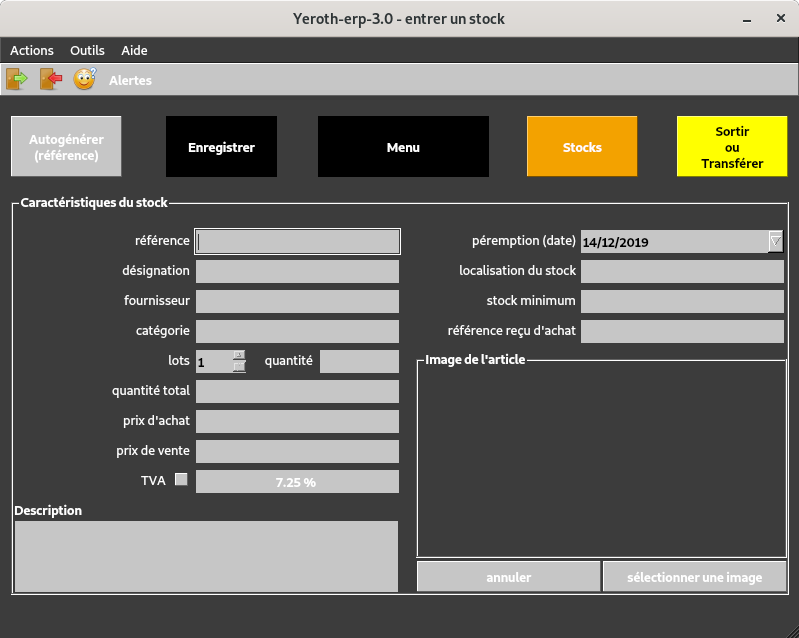
\includegraphics[scale=0.63]{images/yeren-fenetre-entrer.png}
		  \caption{Le formulaire vide pour entrer un stock.}
		  \label{fig:formulaire-entrer-1}
		  \end{figure}	     
	      
	\newpage	      
	      
	\item \textcolor{purplish}{$\mathbf{2^{\text{\`eme}}}$ \textbf{m\'ethode}}
		\begin{enumerate}[1)]
			\item \`A partir de la fen\^etre d'acceuil
			(voir figure~\ref{fig:yeren-fenetre-patron}),
			cliquez sur le boutton \bouton{Stocks}
			\item ensuite, s\'electionnez un stock en cliquant dessus une fois
			\item enfin, cliquez sur le le boutton \bouton{Entrer un stock}.\\
		\end{enumerate}				
		
		L\`a vous obtenez un formulaire partiellement rempli
	    avec les donn\'ees r\'eutilisables du stock s\'electionn\'e.
	    Le formulaire que vous obtenez est celui de la
	    figure~\ref{fig:formulaire-entrer-2}.\\
	    
	    \begin{figure}[!htbp]
		\centering
		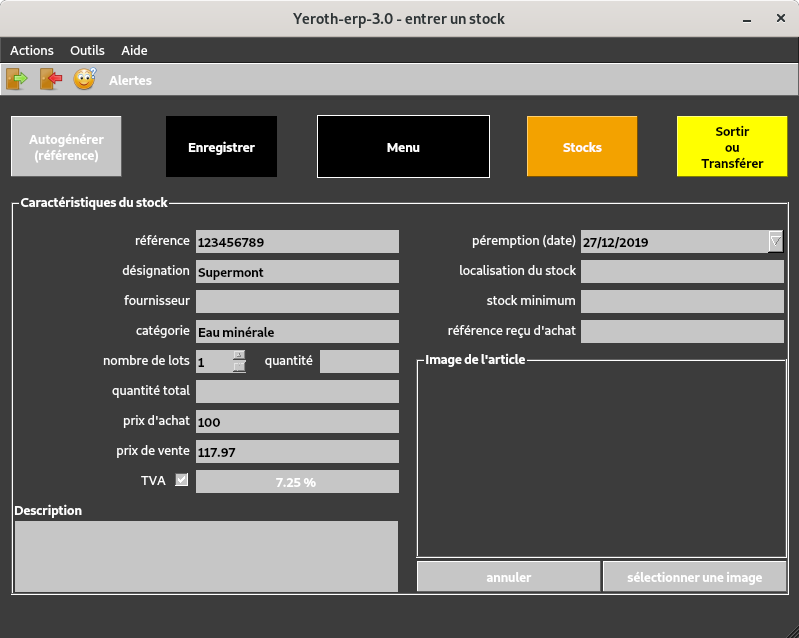
\includegraphics[scale=0.63]{images/yeren-fenetre-entrer-2.png}
		\caption{Le formulaire partiellement rempli pour entrer un nouveau stock.}
		\label{fig:formulaire-entrer-2}
		\end{figure}
\end{itemize}

\newpage

%-----------------------------------------------------------

\nxsection{Lister des stocks}
\index{fiche des stocks}
\index{lister des stocks}
\index{strat\'egie de gestions des stocks}
\index{visualiser la fiche des stocks}
\index{visualiser la liste des stocks}

La figure~\ref{fig:fenetre-lister} illustre la fen\^etre
d'acceuil de \yeren pour lister les stocks.

Le titre de cette fen\^etre explicite la strat\'egie
de gestion des stocks utilis\'ee pour vendre ou
sortir des articles: \cmup.\\

\begin{figure}[!htbp]
\centering
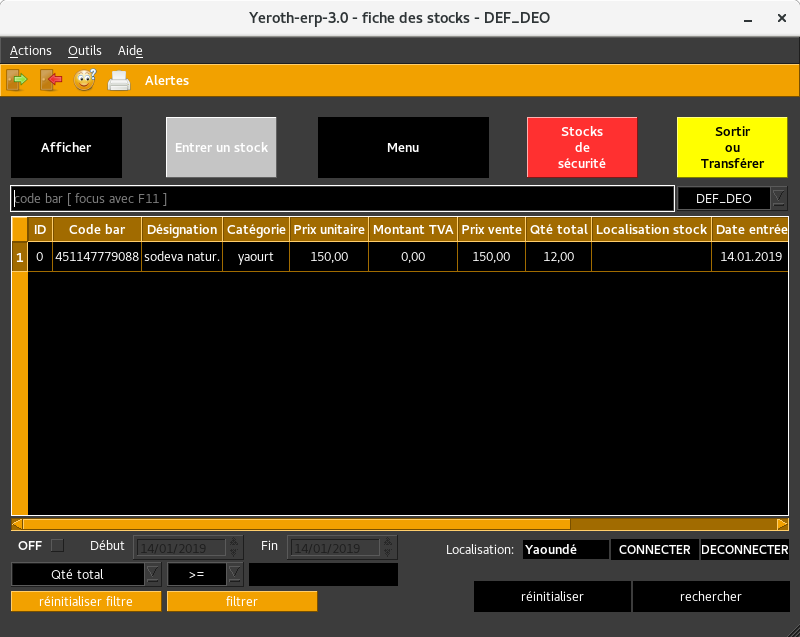
\includegraphics[scale=0.63]{images/yeren-fenetre-lister.png}
\caption{La fen\^etre pour lister les stocks.}
\label{fig:fenetre-lister}
\end{figure}

\`A partir d'une \fenetre quelconque qui y donne
acc\`es, l'acc\`es \`a la fonctionnalit\'e, 'Lister des stocks'
se fait avec au moins l'une des m\'ethodes suivantes: 

\begin{itemize}[\mycheckmark{purplish}]
	\item \textcolor{purplish}{$\mathbf{1^{\text{\`ere}}}$ \textbf{m\'ethode}}\\
		cliquez sur le lien \bouton{Lister des stocks}
		dans le menu d\'eroulant \textbf{Actions}\\

	\item \textcolor{purplish}{$\mathbf{2^{\text{\`eme}}}$ \textbf{m\'ethode}}\\
		cliquez sur le bouton \bouton{Stocks}.
\end{itemize}

\subsection{Les stocks list\'es en rouge}
Les stocks list\'es en \textcolor{firebrickred}{rouge} dans
la colone ''Qt\'e totale'' sont ceux dont la quantit\'e
minimale en stock a \'et\'e atteinte.

Les stocks list\'es en \textcolor{firebrickred}{rouge} dans
la colone ''Date p\'eremption'' sont ceux dont la date de
p\'eremption a \'et\'e atteinte.

\subsection{Les stocks list\'es en vert}
Les stocks list\'es en \textcolor{medgreen}{vert} dans la
colone ''Date p\'eremption'' sont ceux qui ont \'et\'e
s\'electionn\'es pour la vente par l'algorithme correspondant:
\dpfdpo.

Les stocks list\'es en \textcolor{medgreen}{vert} dans la
colone ''Date entr\'ee'' sont ceux qui ont \'et\'e
s\'electionn\'es pour la vente par lun des algorithmes
suivants: \fifo, \lifo.


%-----------------------------------------------------------
\newpage
\nxsection{Imprimer la fiche des stocks
	au format PDF}\label{sec:imprimer-liste-stocks}
\index{imprimer la fiche des stocks}
\index{imprimer la liste des stocks}

Il existe deux m\'ethodes pour imprimer la liste des
stocks qui appara\^it dans la fen\^etre titr\'ee
'\textbf{Yeren - Lister des stocks}'.

\begin{itemize}[\mycheckmark{purplish}]
	\item \textcolor{purplish}{$\mathbf{1^{\text{\`ere}}}$ \textbf{m\'ethode}}\\
		Cliquez sur le lien '\textbf{Imprimer la fiche des stocks}'
		qui se trouve dans le menu d\'eroulant '\textbf{Outils}'\\

	\item \textcolor{purplish}{$\mathbf{2^{\text{\`eme}}}$ \textbf{m\'ethode}}\\
		Cliquez sur l'ic\^one blanche repr\'esentant
		une 'imprimante'\\

	\item \textcolor{purplish}{$\mathbf{3^{\text{\`eme}}}$ \textbf{m\'ethode}}\\
		Pressez simultan\'ement les boutons \bouton{CTRL}
		et \bouton{P} de votre clavier.\\
\end{itemize}

Un fichier au format PDF ayant la liste des stocks affich\'ee
est alors g\'en\'er\'e.

%-----------------------------------------------------------
%\newpage
\nxsection{Rechercher un article ou un stock}
\index{rechercher un article}
\index{rechercher un stock}

Il existe deux m\'etodes pour rechercher un article / stock:
\begin{itemize}[\mycheckmark{purplish}]
	\item \textcolor{purplish}{$\mathbf{1^{\text{\`ere}}}$ \textbf{m\'ethode}}

	\begin{enumerate}[1)]
		\item cliquez sur le bouton \bouton{rechercher}
		\item ou bien cliquez sur le lien '\textbf{Rechercher un article}'
			dans le menu d\'eroulant \textbf{Outils}.\\
	\end{enumerate}
	
	L'utilisateur est alors conduit vers une petite fen\^etre de
	dialogue ou il peut introduire les mots cl\'es de sa recherche,
	ainsi que les param\`etres optionels suivants: la
	\yerenfield{cat\'egorie du stock}, la \yerenfield{d\'esignation du stock}
	et le \yerenfield{fournisseur du stock}.
	Ceci est illustr\'e dans la figure~\ref{fig:fenetre-rechercher-stock}.\\
	
	\begin{figure}[!htbp]
		\centering
		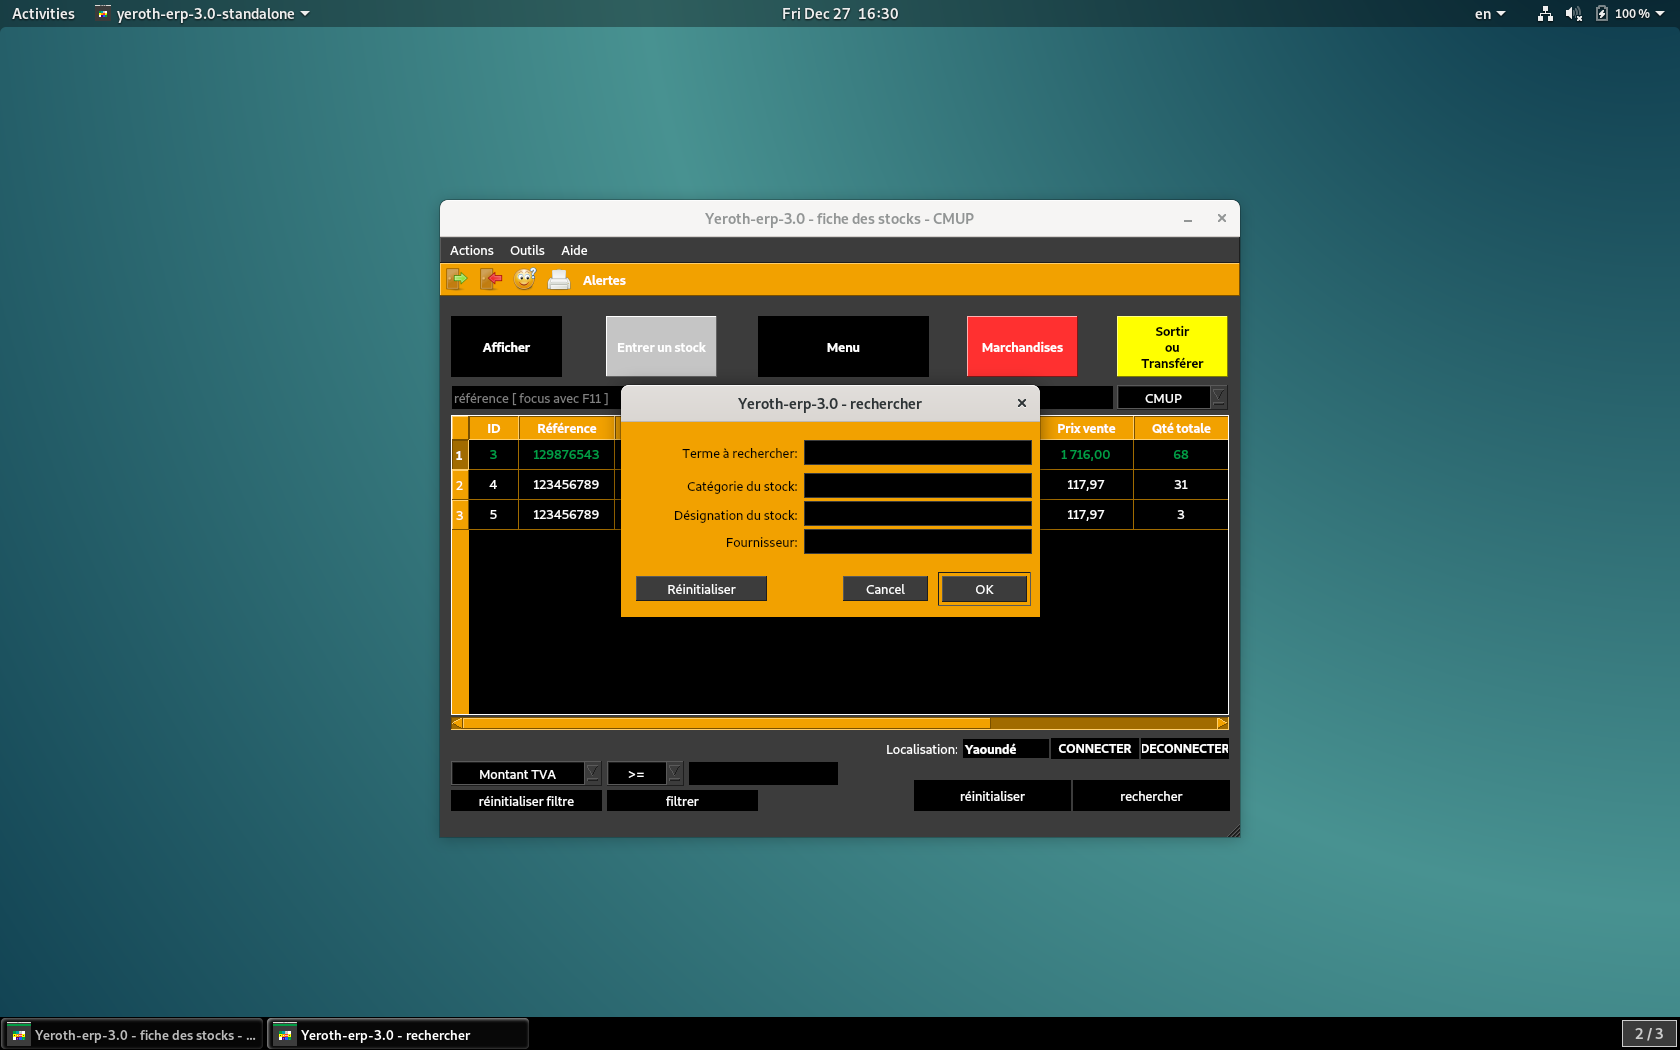
\includegraphics[scale=0.26]{images/yeren-rechercher-un-article.png}
		\caption{La fen\^etre pour rechercher un stock (ou un article).}
		\label{fig:fenetre-rechercher-stock}
	\end{figure}
	
	Pour une recheche efficace, les mots cl\'es doivent \^etre des
	mots ou parcelle de mots qui appara\^issent dans les endroits
	suivant:
	\begin{enumerate}[1)]
		\item la cat\'egorie du stock
		\item la d\'esignation du fournisseur		
		\item la d\'esignation du stock
		\item les mots qui ont \'et\'e introduits dans
			le champs de texte '\textbf{Description}'
			qui appara\^it lorsque l'on entre un nouveau stock
			(voir par example le figure~\ref{fig:formulaire-entrer-2}).
	\end{enumerate}
		
	\newpage	
	
	\item \textcolor{purplish}{$\mathbf{2^{\text{\`eme}}}$ \textbf{m\'ethode}}\\
	L'utilisateur peut aussi entrer la r\'ef\'erence
	du stock recherch\'e dans le champs	de recherche
	situ\'e juste en dessous des boutons
	suivants: \bouton{Afficher}, \bouton{Entrer un nouveau stock},
	\bouton{Menu}, \bouton{Modifier}, et \bouton{Sortir}.\\
		
	\begin{figure}[!htbp]
		\centering
		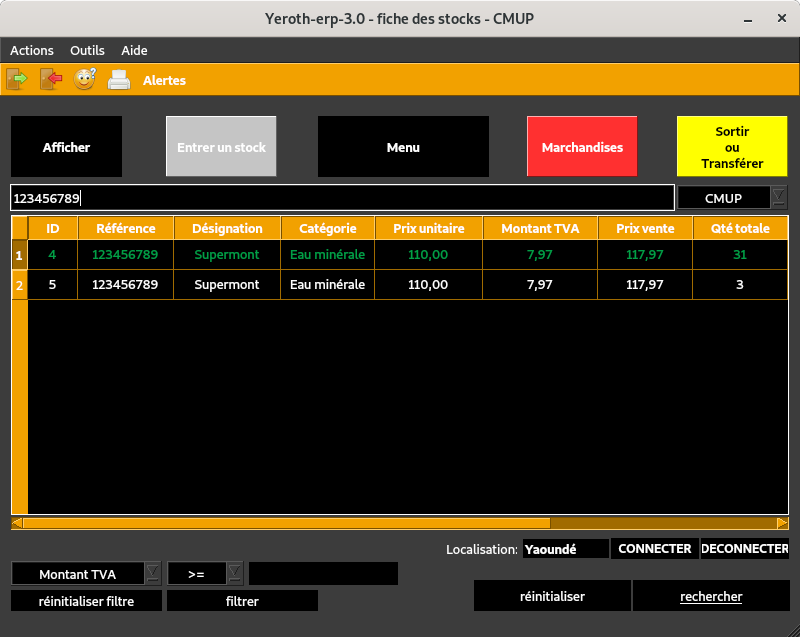
\includegraphics[scale=0.63]{images/yeren-fenetre-rechercher-stock-par-reference.png}
		\caption{Le champs de texte pour
			rechercher les stocks (ou articles) en utilisant
			seulement leur r\'ef\'erence.}\label{fig:yeren-fenetre-rechercher-stock-par-reference}
	\end{figure}
	
	Ceci est illustr\'e dans la figure~\ref{fig:yeren-fenetre-rechercher-stock-par-reference}
	o\`u les stocks ayant la r\'ef\'erence '\textbf{123456789}'
	ont \'et\'e recherch\'es.\\	
\end{itemize}

Lorsqu'une recherche de stocks (ou d'articles) est active,
le mot 'rechercher' du bouton \bouton{rechercher} et
le lien '\textbf{Rechercher un article}' dans le
menu d\'eroulant '\textbf{Outils}' sont soulign\'es.
	
Le bouton \bouton{r\'einitialiser} ou le lien
'\textbf{R\'einitialiser la recherche}' dans le menu 
d\'eroulant '\textbf{Outils}' permettent de d\'eactiver
la recherche et ainsi d'afficher tous les stocks
\`a nouveau.

%-----------------------------------------------------------
\newpage
\nxsection{Afficher les d\'etails d'un stock}
\index{afficher les d\'etails d'un stock}

La figure~\ref{fig:fenetre-details-stock} illustre
les d\'etails du stock '\textbf{Supermont}'.\\

\begin{figure}[!htbp]
	\centering
	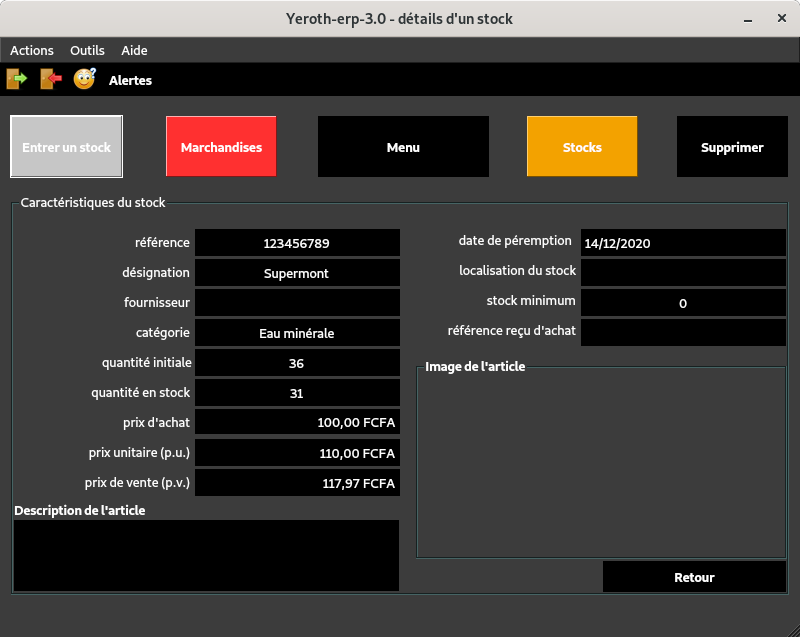
\includegraphics[scale=0.63]{images/yeren-fenetre-detail-stock.png}
	\caption{Une fen\^etre qui pr\'esente les d\'etails d'un stock.}
	\label{fig:fenetre-details-stock}
\end{figure}

Il existe trois m\'ethodes pour afficher les d\'etails
d'un stock:

\begin{itemize}[\mycheckmark{purplish}]
	\item \textcolor{purplish}{$\mathbf{1^{\text{\`ere}}}$ \textbf{m\'ethode}}
		\begin{enumerate}[1)]
			\item s\'electionnez le stock dont vous souhaitez
			afficher les d\'etails en cliquant une fois sur lui
			\` a partir de la fen\^etre '\textbf{fiche des stocks}'
			
			\item cliquez ensuite sur le bouton \bouton{Afficher}.	\\
		\end{enumerate}
	
	\item \textcolor{purplish}{$\mathbf{2^{\text{\`eme}}}$ \textbf{m\'ethode}}
		\begin{enumerate}[1)]
			\item s\'electionner le stock dont vous souhaitez
			afficher les d\'etails en cliquant une fois sur lui
			\` a partir de la fen\^etre '\textbf{fiche des stocks}'
			
			\item cliquer ensuite sur le lien '\textbf{Afficher les d\'etails de ce stock}'
			du menu d\'eroulant \textbf{Actions}.\\
		\end{enumerate}
	
	\item \textcolor{purplish}{$\mathbf{3^{\text{\`eme}}}$ \textbf{m\'ethode}}
		\begin{enumerate}[1)]
			\item s\'electionner le stock dont vous souhaitez
			afficher les d\'etails en cliquant une fois sur lui
			\` a partir de la fen\^etre '\textbf{fiche des stocks}'
			
			\item maintener l'indexeur de la souris sur le stock
				s\'electionner et ensuite cliquer sur le bouton
				droit de la souris
			
			\item un menu d\'eroulant s'affiche, cliquer sur
				le lien '\textbf{Afficher les d\'etails de ce stock}' du
				menu d\'eroulant qui s'est affich\'e. 
		\end{enumerate}
\end{itemize}

%-----------------------------------------------------------
\newpage
\nxsection{Consulter l'historique d'un stock}
\index{consulter l'historique d'un stock}
\index{l'historique d'un stock}

La figure~\ref{fig:fenetre-historique-dun-stock}
illustre l'historique d'un stock.

\begin{figure}[!htbp]
	\centering
	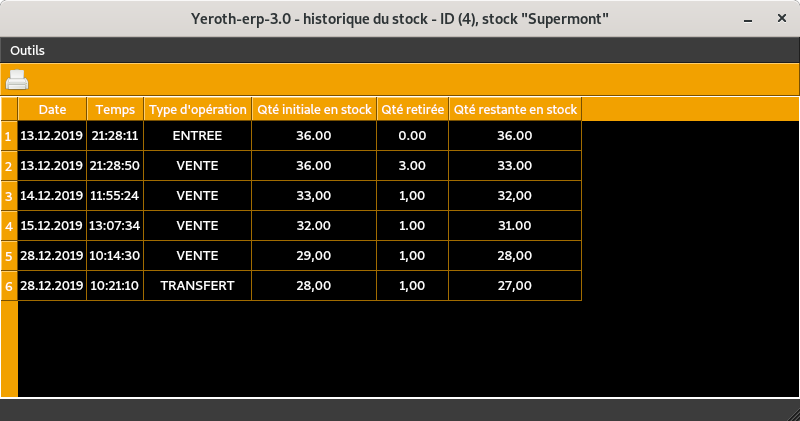
\includegraphics[scale=0.63]{images/yeroth-historique-stock.png}
	\caption{L'historique d'un stock.}
	\label{fig:fenetre-historique-dun-stock}
\end{figure}

\begin{itemize}[\mycheckmark{purplish}]
	\item \textcolor{purplish}{$\mathbf{1^{\text{\`ere}}}$ \textbf{m\'ethode}}
	\begin{enumerate}[1)]
		\item s\'electionner le stock dont vous souhaitez
		consulter l'historique en cliquant sur lui avec
		le boutton gauche de la souris
		\` a partir de la fen\^etre '\textbf{fiche des stocks}'
		
		\item cliquer ensuite sur le lien
		 '\textbf{Afficher l'historique de ce stock}' du
		 menu d\'eroulant \textbf{Actions}.\\
	\end{enumerate}
	
	\item \textcolor{purplish}{$\mathbf{2^{\text{\`eme}}}$ \textbf{m\'ethode}}
	\begin{enumerate}[1)]
		\item s\'electionner le stock dont vous souhaitez
		consulter l'historique en cliquant sur lui avec
		le boutton droit de la souris
		\` a partir de la fen\^etre '\textbf{fiche des stocks}'
		
		\item cliquer ensuite sur le lien
		 '\textbf{Afficher l'historique de ce stock}' du
		 menu contextuel qui s'est affich\'e.\\
	\end{enumerate}
	
\end{itemize}

L'historique du stock peut \^etre imprim\'e
au format PDF en cliquant sur l'ic\^one
repr\'esentant une imprimante.


%-----------------------------------------------------------
\newpage
\nxsection{Modifier les d\'etails d'un stock}
\index{modifier les d\'etails d'un stock}

La figure~\ref{fig:yeren-fenetre-modifier-stock}
illustre la fen\^etre pour modifier les d\'etails
du stock '\textbf{Cola}'.\\

\begin{figure}[!htbp]
	\centering
	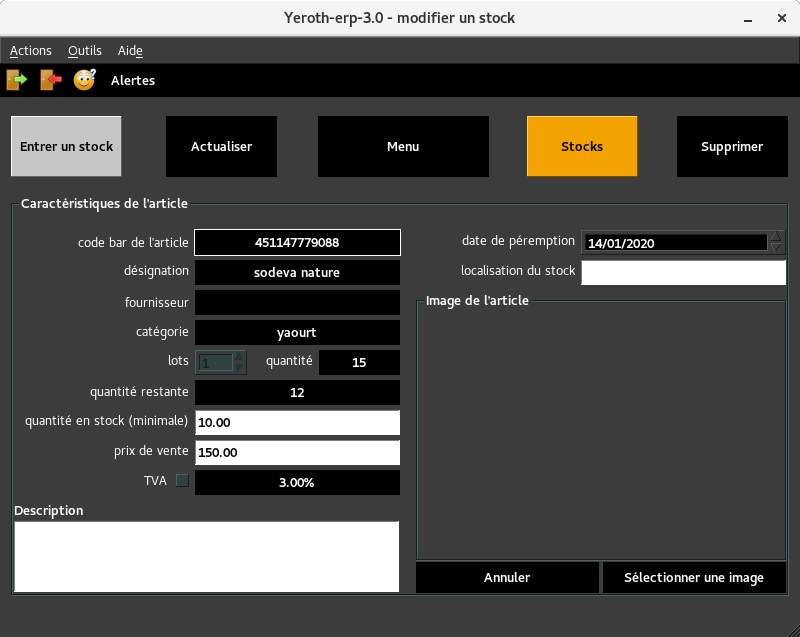
\includegraphics[scale=0.63]{images/yeren-fenetre-modifier-stock.png}
	\caption{Une fen\^etre qui permet la modification des d\'etails d'un stock.}
	\label{fig:yeren-fenetre-modifier-stock}
\end{figure}

Seul les informations suivantes d'un stock peuvent
\^etre modifi\'ees:
\begin{enumerate}[1)]
	\item la date de p\'eremption des articles du stock
	\item la quantit\'e minimale en stock
	\item le prix de vente d'un article du stock.\\
\end{enumerate}

Il existe trois m\'ethodes pour modifier les d\'etails
d'un stock:

\begin{itemize}[\mycheckmark{purplish}]
	\item \textcolor{purplish}{$\mathbf{1^{\text{\`ere}}}$ \textbf{m\'ethode}}
	\begin{enumerate}[1)]
		\item s\'electionner le stock dont vous souhaitez
		modifier les d\'etails en cliquant une fois sur lui
		\` a partir de la fen\^etre '\textbf{fiche des stocks}'
		
		\item cliquer ensuite sur le bouton \bouton{Modifier}.	\\
	\end{enumerate}
	
	\item \textcolor{purplish}{$\mathbf{2^{\text{\`eme}}}$ \textbf{m\'ethode}}
	\begin{enumerate}[1)]
		\item s\'electionner le stock dont vous souhaitez
		modifier les d\'etails en cliquant une fois sur lui
		\` a partir de la fen\^etre '\textbf{fiche des stocks}'
		
		\item cliquer ensuite sur le lien '\textbf{Modifier ce stock}'
		du menu d\'eroulant \textbf{Actions}.\\
	\end{enumerate}
	
	\item \textcolor{purplish}{$\mathbf{3^{\text{\`eme}}}$ \textbf{m\'ethode}}
	\begin{enumerate}[1)]
		\item s\'electionner le stock dont vous souhaitez
		modifier les d\'etails en cliquant une fois sur lui
		\` a partir de la fen\^etre '\textbf{fiche des stocks}'
		
		\item maintener l'indexeur de la souris sur le stock
		s\'electionn\'e et ensuite cliquer sur le bouton
		droit de la souris
		
		\item un menu d\'eroulant s'affiche, cliquer sur
		le lien '\textbf{Modifier ce stock}' du	menu
		d\'eroulant qui s'est affich\'e.\\
	\end{enumerate}
\end{itemize}

%-----------------------------------------------------------

\newpage
\nxsection{Visualiser les articles / stocks p\'erim\'es}
\index{visualiser les articles p\'erim\'es}
\index{visualiser les stocks p\'erim\'es}

La figure~\ref{fig:fenetre-lister-stock-perime} illustre
que la date de p\'eremption du stock 'Cola' ($22$ F\'evrier
$2017$) est d\'epass\'ee.\\

\begin{figure}[!htbp]
	\centering
	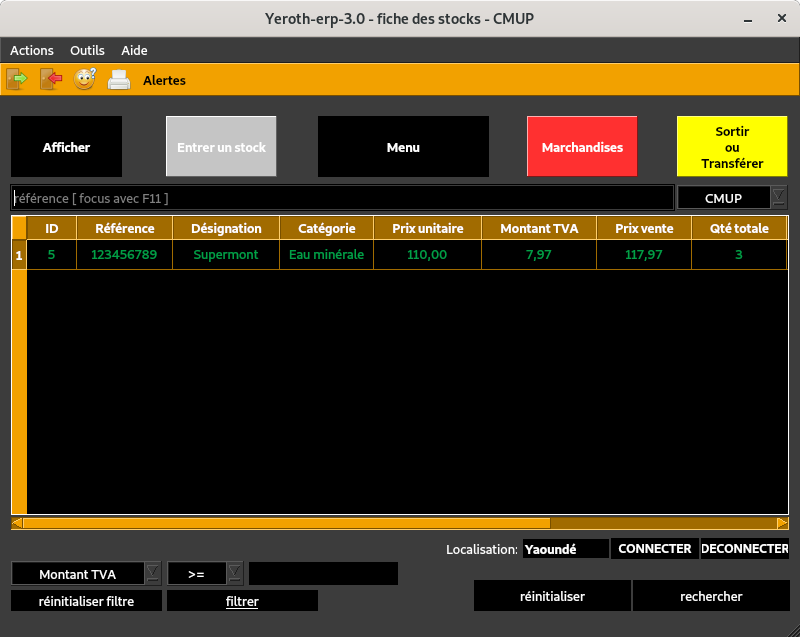
\includegraphics[scale=0.63]{images/yeren-fenetre-stocks-perimes.png}
	\caption{Le stock 'Cola' est p\'erim\'e.}
	\label{fig:fenetre-lister-stock-perime}
\end{figure}

On visualise les stocks p\'erim\'es en allant \`a la fen\^etre
'\textbf{fiche des stocks}'. 

Tous les stocks dont la colone '\textbf{Date de
	p\'eremption}' est affich\'ee en 
\textbf{\textcolor{firebrickred}{rouge}} sont p\'erim\'es.

%-----------------------------------------------------------

\newpage
\nxsection{Visualiser les stocks dont la quantit\'e minimale 
	en stock est atteinte}
\index{la quantit\'e minimale en stock est atteinte}

L'utilisateur de \yeren peut d\'efinir une quantit\'e minimale
pour un stock: c'est \emph{le nombre d'articles du stock en dessous
duquel l'entreprise ne devrait pas se retrouver}.

La figure~\ref{fig:fenetre-lister-quantite-minimale} illustre
que la quantit\'e minimale de $50$ articles du stock 'Cola'
est atteinte.\\

\begin{figure}[!htbp]
	\centering
	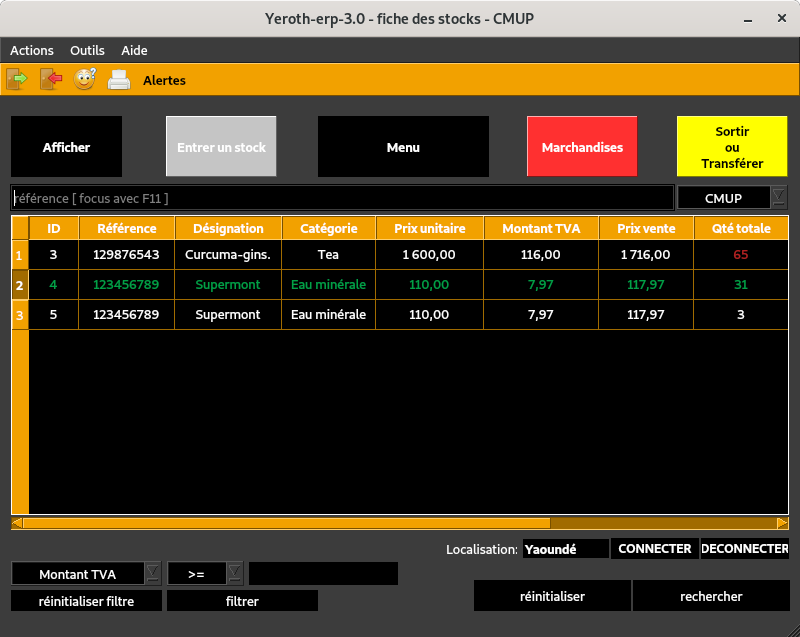
\includegraphics[scale=0.63]{images/yeren-fenetre-stock-minimal-atteint.png}
	\caption{La quantit\'e minimale du stock 'Cola' est atteinte.}
	\label{fig:fenetre-lister-quantite-minimale}
\end{figure}

On visualise les stocks dont la quantit\'e minimale en stock
est atteinte en allant \`a la fen\^etre '\textbf{fiche des stocks}'.

Tous les stocks dont la colone '\textbf{Quantit\'e en stock}'
est affich\'ee en \textbf{\textcolor{firebrickred}{rouge}}
ont leur quantit\'e minimale en stock d\'ej\`a ateinte.

%-----------------------------------------------------------

%\newpage
\nxsection{Supprimer un stock}
\index{supprimer un stock}

Il existe deux m\'etodes pour supprimer un stock:
\begin{itemize}[\mycheckmark{purplish}]
	\item \textcolor{purplish}{$\mathbf{1^{\text{\`ere}}}$ \textbf{m\'ethode}}
	
	\begin{enumerate}[1)]
		\item s\'electionner le stock \`a supprimer partir de
		la fen\^etre '\textbf{fiche des stocks}'
		
		\item cliquer ensuite sur le lien '\textbf{Supprimer ce stock}'
		dans le menu d\'eroulant \textbf{Actions}.\\
	\end{enumerate}
	
	\item \textcolor{purplish}{$\mathbf{2^{\text{\`eme}}}$ \textbf{m\'ethode}}
	\begin{enumerate}[1)]
		\item s\'electionner le stock \`a supprimer partir de
			la fen\^etre '\textbf{fiche des stocks}'
		
		\item maintener l'indexeur de la souris sur le stock
			s\'electionn\'e et ensuite cliquer sur le bouton
			droit de la souris
				
		\item un menu d\'eroulant s'affiche, cliquer sur
			le lien '\textbf{Supprimer ce stock}' du menu
			d\'eroulant qui s'est affich\'e. \\
	\end{enumerate}	
\end{itemize}

Le stock supprim\'e n'est plus affich\'e.

\chapter{La Gestion des Achats}
\label{chap:gestion-des-achats}




\begin{figure}[!htbp]
\centering
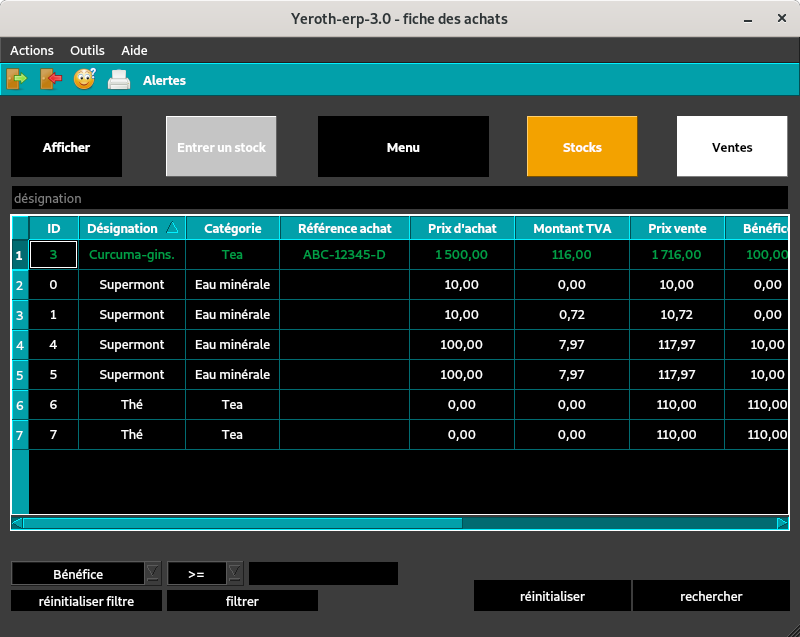
\includegraphics[scale=0.63]{images/yeroth-lister-des-achats.png}
\caption{La fen\^etre pour lister des achats.}
\label{fig:fenetre-lister-des-achats}
\end{figure}
\chapter{Le Syst\`eme d'Alertes sur les Stocks}\label{chap:systeme-dalertes}
\index{syst\`eme d'alertes}

\utilisateurs: \lienadmin, \liencaissier, \lienmagasinier, \lienpatron.\\

\chapintro{Ce chapitre d\'ecrit comment cr\'eer, lister, modifier,
et supprimer les alertes sur les stocks.}

\nxsection{Introduction}

Le programme qui impl\'emente le syst\`eme d'alertes
de \yeren s'appelle ''\emphbf{yeren-alert}''.

\yerenalert est configur\'e pour d\'emarrer en tant que
''\emphbf{processus en arri\`ere plan}'' lors du
d\'emarrage de l'ordinateur.

La figure~\ref{fig:yeren-fenetre-creer-alerte}
pr\'esente l'interface graphique de \yeren pour
cr\'eer une alerte.

\begin{figure}[!htbp]
	\centering
	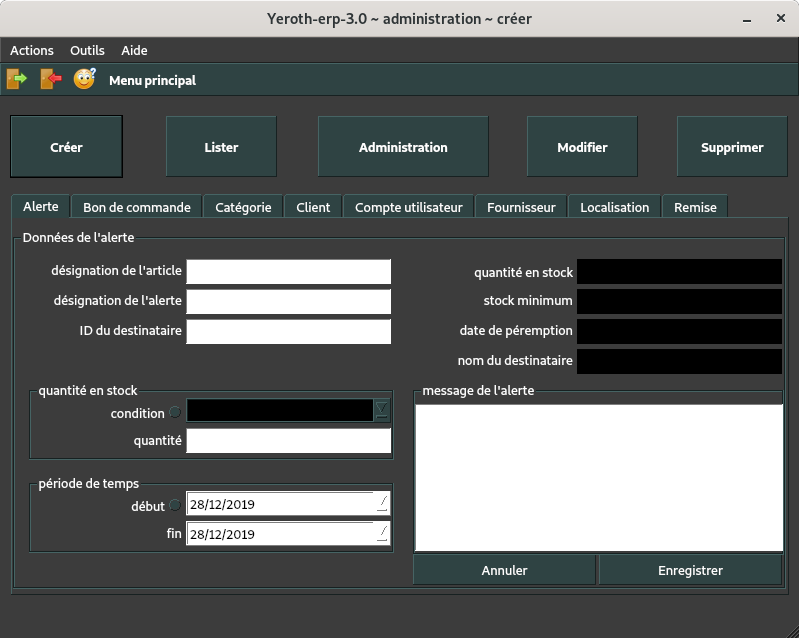
\includegraphics[scale=0.63]{images/yeren-fenetre-creer-alerte.png}
	\caption{La fen\^etre principale pour la cr\'eation d'une alerte.}
	\label{fig:yeren-fenetre-creer-alerte}
\end{figure}

le syst\`eme d'alertes sur les stocks permet aux
utilisateurs de contr\^oler \emph{les dates de
p\'eremption des stocks},
ainsi que \emph{les quantit\'es d'articles en stock}.

\yeren d\'efinit deux types d'alertes sur les stocks:
\begin{enumerate}[1)]
	\item \textbf{les alertes sur une quantit\'e en stock}
	\item \textbf{les alertes sur une p\'eriode de temps}.\\
\end{enumerate}

L'interface de \yeren pour cr\'eer des alertes a deux
\emph{boutons de radio}~\footnote{les boutons de radio
	permettent de faire des choix exclusifs}:

\begin{enumerate}[1)]
	\item le bouton de radio 'quantit\'e en stock'
	\item le bouton de radio 'p\'eriode de temps'.
\end{enumerate}

%-----------------------------------------------------------

\newpage
\nxsection{Cr\'eer une alerte sur une quantit\'e en stock}\label{sec:alerte-quantite-stock}
\index{cr\'eer une alerte sur une quantit\'e en stock}

\begin{enumerate}[1)]
	\item \`A partir de l'interface graphique de l'acceuil de
		l'administration (voir figure~\ref{fig:fenetre-administrateur}),
		on clique sur l'onglet intitul\'e \textbf{op\'erations}. 
		
	\item Choisir '\textbf{cr\'eer}' dans le '\emph{combo box
		op\'erations}'.
		
	\item Choisir '\textbf{une alerte}' dans le '\emph{combo box
		sujets}'. Vous \^etes automatiquement conduit \`a la fen\^etre
		illustr\'ee sur la figure~\ref{fig:yeren-fenetre-creer-alerte}.	
		
	\item Il est pr\'ef\'erable pour de d'abord	choisir le stock
		pour lequel une alerte doit \^etre cr\'eer.	Pour cela il
		faut choisir sa d\'esignation dans le champs de texte
		'\textbf{d\'esignation de l'article}', qui poss\`ede un
		menu auto-d\'eroulant.\\

		Les informations des champs de textes situ\'ees \`a
		droite du champs de texte '\textbf{d\'esignation de l'article}'
		sont non modifiables et affichent des valeurs en fonction
		du stock de l'article s\'electionn\'e:
		\begin{enumerate} [1)]
			\item quantit\'e en stock
			\item quantit\'e minimale (stock)
			\item date de p\'eremption.		
		\end{enumerate}

		Ces informations aident \`a param\'etrer l'alerte.

	\item Donner une d\'esignation \`a l'alerte	en remplissant
		le champs de texte '\textbf{d\'esignation de l'alerte}'.
		
	\item Choisir un destinataire qui recevra le message de
		l'alerte lorsque celle-ci sera d\'eclench\'ee.
		Ceci se fait dans le champs de texte '\textbf{ID du destinataire}',
		qui poss\`ede un menu auto-d\'eroulant.\\
		
		Le nom complet du destinataire est affich\'e automatiquement
		dans le champs de texte '\textbf{nom du destinataire}',
		qui est situ\'e juste \`a droite du champs de texte
		'\textbf{ID du destinataire}'.
		
	\item Choisir le type d'alerte:	\emphbf{quantit\'e en stock}
		en cliquant sur la bouton radio '\textbf{condition}' et 
		en \emph{saisissant un nombre dans le champs de texte
		'\textbf{quantit\'e}'}.
		
	\item Remplir le champs de texte '\textbf{Message de l'alerte}'.
		C'est ce message qui sera envoy\'e au destinataire de
		l'alerte lorsque celle-ci sera d\'eclench\'ee.	
		
	\item Achever la proc\'edure en cliquant sur le bouton \bouton{Valider}.
\end{enumerate}

%-----------------------------------------------------------

\newpage
\nxsection{Cr\'eer une alerte sur une p\'eriode de temps}\label{sec:alerte-periode-temps}
\index{cr\'eer une alerte sur une p\'eriode de temps}

\begin{enumerate}[1)]
	\item \`A partir de l'interface graphique de l'acceuil de
		l'administration (voir figure~\ref{fig:fenetre-administrateur}),
		on clique sur l'onglet intitul\'e \textbf{op\'erations}. 
		
	\item Choisir '\textbf{cr\'eer}' dans le '\emph{combo box
		op\'erations}'.
		
	\item Choisir '\textbf{une alerte}' dans le '\emph{combo box
		sujets}'. Vous \^etes automatiquement conduit \`a la fen\^etre
		illustr\'ee sur la figure~\ref{fig:yeren-fenetre-creer-alerte}.	
		
	\item Il est pr\'ef\'erable pour de d'abord	choisir le stock
		pour lequel une alerte doit \^etre cr\'eer.	Pour cela il
		faut choisir sa d\'esignation dans le champs de texte
		'\textbf{d\'esignation de l'article}', qui poss\`ede un
		menu auto-d\'eroulant.\\

		Les informations des champs de textes situ\'ees \`a
		droite du champs de texte '\textbf{d\'esignation de l'article}'
		sont non modifiables et affichent des valeurs en fonction
		du stock de l'article s\'electionn\'e:
		\begin{enumerate} [1)]
			\item quantit\'e en stock
			\item quantit\'e minimale (stock)
			\item date de p\'eremption.		
		\end{enumerate}

		Ces informations aident \`a param\'etrer l'alerte.

	\item Donner une d\'esignation \`a l'alerte	en remplissant
		le champs de texte '\textbf{d\'esignation de l'alerte}'.
		
	\item Choisir un destinataire qui recevra le message de
		l'alerte lorsque celle-ci sera d\'eclench\'ee.
		Ceci se fait dans le champs de texte '\textbf{ID du destinataire}',
		qui poss\`ede un menu auto-d\'eroulant.\\
		
		Le nom complet du destinataire est affich\'e automatiquement
		dans le champs de texte '\textbf{nom du destinataire}',
		qui est situ\'e juste \`a droite du champs de texte
		'\textbf{ID du destinataire}'.
		
	\item Choisir le type d'alerte:	\emphbf{p\'eriode de temps}
		en cliquant sur la bouton radio '\textbf{d\'ebut}' et 
		en choisissant \emph{les dates de d\'ebut et de fin de
		la p\'eriode de temps pendant laquelle l'alerte sera active}.
		
	\item Remplir le champs de texte '\textbf{Message de l'alerte}'.
		C'est ce message qui sera envoy\'e au destinataire de
		l'alerte lorsque celle-ci sera d\'eclench\'ee.	
		
	\item Achever la proc\'edure en cliquant sur le bouton \bouton{Valider}.
\end{enumerate}

%-----------------------------------------------------------

\newpage
\nxsection{Voir toutes les alertes qu'un utilisateur
 a re\c{c}u~\textcolor{blue}{*}}\label{sec:voire-toutes-alertes}
\index{voir toutes les alertes qu'un utilisateur a re\c{c}u }

\textcolor{blue}{*: Cette fonctionalit\'e est exclusivement
	r\'eserv\'ee aux utilisateurs \patron.}

Pour voire toutes les alertes qui lui sont destin\'ees, l'utilisateur
doit accomplir les actions suivantes \`a partir de toutes fen\^etre
ayant le lien '\textbf{Alertes}' dans sa barre de menu:
\begin{enumerate}[1)]
	\item cliquer sur le lien '\textbf{Alertes}' qui est situ\'e
	dans la barre de menu. Ce lien se retrouve dans toutes les
	fen\^etres concernant la gestion des stocks
	
	\item un utilisateur a aussi acc\`es aux alertes qui lui sont destin\'ees en cliquant sur le lien '\textbf{Alertes}' que
	l'on retrouve dans le menu d\'eroulant \textbf{Outils}.
\end{enumerate}

%-----------------------------------------------------------

\nxsection{Voir les d\'etails d'une alerte}\label{sec:voire-details-alerte}
\index{voir les d\'etails d'une alerte}

L'utilisateur doit accomplir les actions suivantes \`a
partir de toutes fen\^etre ayant le lien '\textbf{Alertes}'
dans sa barre de menu:

\begin{enumerate}[1)]
	\item cliquer sur le lien '\textbf{Alertes}' qui est situ\'e
	dans la barre de menu. Ce lien se retrouve dans toutes les
	fen\^etres concernant la gestion des stocks
		
	\item ensuite, s\'electioner dans l'onglet '\textbf{Alertes}'
		l'alerte dont vous souhaiter voire les d\'etails

	\item enfin, cliquer 2 fois cons\'ecutives sur cette alerte.	
\end{enumerate}

%-----------------------------------------------------------

\nxsection{Marquer une alerte comme r\'esolue~\textcolor{blue}{*}}
\index{marquer une alerte comme r\'esolue}

\textcolor{blue}{*: Cette fonctionalit\'e est exclusivement
	r\'eserv\'ee aux utilisateurs \patron.}

L'utilisateur doit accomplir les actions suivantes \`a
partir de toutes fen\^etre ayant le lien '\textbf{Alertes}'
dans sa barre de menu:

\begin{enumerate}[1)]
	\item cliquer sur le lien '\textbf{Alertes}' qui est situ\'e
	dans la barre de menu. Ce lien se retrouve dans toutes les
	fen\^etres concernant la gestion des stocks
		
	\item ensuite, s\'electioner dans l'onglet '\textbf{Alertes}'
		l'alerte dont vous souhaiter voire les d\'etails

	\item enfin, cliquez sur le bouton \bouton{Marquer r\'esolue}.	
\end{enumerate}

%-----------------------------------------------------------
\newpage
\nxsection{Supprimer une alerte~\textcolor{blue}{*}}
\index{supprimer une alerte}

\textcolor{blue}{*: Cette fonctionalit\'e est exclusivement
		r\'eserv\'ee aux utilisateurs \patron.}

L'utilisateur doit accomplir les actions suivantes \`a
partir de toutes fen\^etre ayant le lien '\textbf{Alertes}'
dans sa barre de menu:

\begin{enumerate}[1)]
	\item cliquer sur le lien '\textbf{Alertes}' qui est situ\'e
	dans la barre de menu. Ce lien se retrouve dans toutes les
	fen\^etres concernant la gestion des stocks
		
	\item ensuite, s\'electioner dans l'onglet '\textbf{Alertes}'
		l'alerte dont vous souhaiter voire les d\'etails

	\item enfin, cliquez sur le bouton \bouton{Supprimer une alerte}.
\end{enumerate}

\chapter{La Sortie d'Articles}\label{chap:sortir-articles}
\index{la sortie d'articles}
\index{la sortie de stocks}

\utilisateurs: \lienmagasinier, \lienpatron.\\

\chapintro{Ce chapitre d\'ecrit comment proc\'eder \`a la
sortie ou au transfert d'articles.}

\nxsection{Introduction}

\begin{figure}[!htbp]
	\centering
	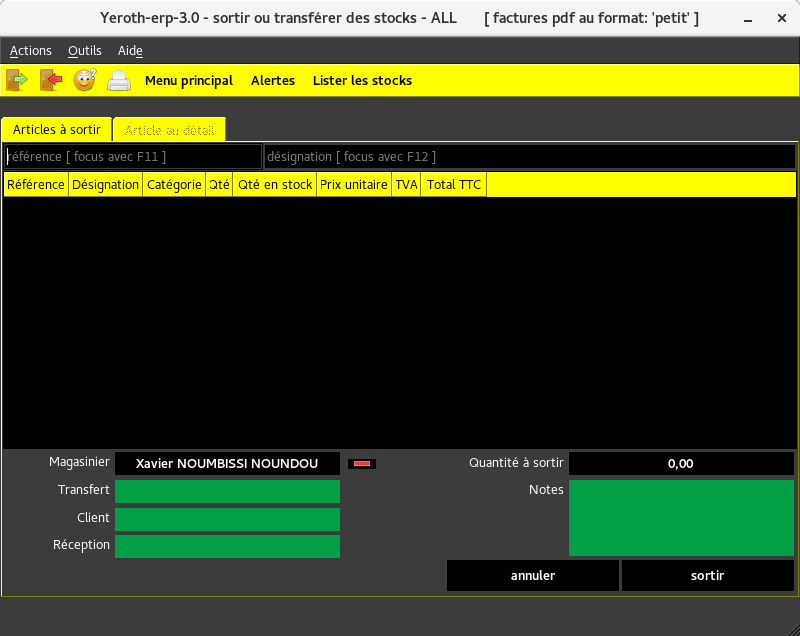
\includegraphics[scale=0.63]{images/yeren-fenetre-sortir-articles.png}
	\caption{La fen\^etre pour sortir des articles en stock.}
	\label{fig:yeren-fenetre-sortir-articles}
\end{figure}

La figure~\ref{fig:yeren-fenetre-sortir-articles} illustre
l'interface graphique pour proc\'eder aux sorties, ou aux
transferts d'articles.

La fen\^etre avec pour titre ''sortir ou transf\'erer des stocks''
permet d'effectuer les op\'erations suivantes:
\begin{enumerate}[1)]
	\item \textbf{une sortie de stocks};
	\item \textbf{un transfert de stocks}.\\
\end{enumerate}

Une \textbf{sortie de stocks} est le retrait d'articles
par un client aupr\`es d'une boutique (ou d'un d\'ep\^ot)
de votre entreprise apr\`es que le paiement se soit
effectu\'e dans une autre unit\'e de l'entreprise.

Un \textbf{transfert de stocks} est un mouvement de stocks
d'une boutique (ou d'un d\'ep\^ot) de votre entreprise
vers une autre unit\'e de l'entreprise.

\subsection{La strat\'egie de sortie des articles / stocks utilis\'ee}
\index{La strat\'egie de sortie des articles}
\index{La strat\'egie de sortie des stocks}

Le titre de la fen\^etre affiche la strat\'egie de sortie
des stocks utilis\'ee. La strat\'egie affich\'ee dans la
figure~\ref{fig:yeren-fenetre-sortir-articles} est: ''\cmup''
(en effet: \textbf{Cours Moyen Unit\'e Pond\'er\'e}).

%---------------------------------------------------

\nxsection{Effectuer une sortie d'articles}
\index{effectuer une sortie d'articles}
\index{effectuer une sortie de stock}

La d\'emarche pour effectuer une sortie d'articles en stock
est la suivante:
\begin{enumerate}[1)]
	\item s\'electionner les articles \`a faire sortir
	(appliquer l'une des m\'ethodes d\'ecrites dans
	la section~\ref{sec:selectionner-articles-vendre}
	du chapitre~\ref{chap:vendre} sur la vente d'article)

	\item le cas \'ech\'eant, choisissez le nom de
	l'entreprise cliente dans le menu d\'eroulant
	du champs de texte '\textbf{Client}'
	
	\item saisissez dans le champs de texte '\textbf{R\'ecepteur}'
	le nom de la personne qui r\'eceptionne les articles
	
	\item si vous avez des notes sp\'ecifiques \`a
	cette sortie d'articles, ecriver les dans 
	le champs de texte '\textbf{notes}'
	
	\item cliquer sur le bouton \bouton{Sortir}
	pour conclure la sortie de stocks.
\end{enumerate}

%---------------------------------------------------

\nxsection{Effectuer un transfert d'articles}
\index{effectuer un transfert d'articles}
\index{effectuer un transfert de stock}

La d\'emarche pour effectuer un transfert d'articles en stock
est la suivante:
\begin{enumerate}[1)]
	\item s\'electionner les articles \`a transf\'erer
	(appliquer l'une des m\'ethodes d\'ecrites dans la
	section~\ref{sec:selectionner-articles-vendre}
	du chapitre~\ref{chap:vendre} sur la vente d'article)
		
	\item saisissez dans le champs de texte
	'\textbf{R\'ecepteur}' le nom de la personne
	qui r\'eceptionne les articles
	
	\item sasissez ensuite dans le champs de texte
	'\textbf{Transfert}' le nom de la boutique ou
	du d\'ep\^ot qui recevra les articles \`a transferer
	
	\item si vous avez des notes sp\'ecifiques \`a
	ce transfert d'articles, ecriver les dans 
	le champs de texte '\textbf{notes}'
	
	\item cliquez sur bouton \bouton{Sortir}
	pour conclure le transfert d'articles.
\end{enumerate}

%---------------------------------------------------

\nxsection{Autres op\'erations de sortie d'articles / de stocks}
\index{autres op\'erations de sortie d'articles}
\index{autres op\'erations de sortie de stocks}

Pour toutes autres op\'erations de sortie des stocks,
appliquer la m\'ethode similaire d\'ecrite dans le
chapitre~\ref{chap:vendre} qui porte sur la vente d'articles
(ex.: annuler la sortie d'articles, imprimer une proforma
du bon de sortie, etc.).

\chapter{Les Transactions (les \'etats de sorties
	d'articles)}\label{chap:etats-des-sorties}

\utilisateurs: \lienmagasinier, \lienmanager.\\

\chapintro{Ce chapitre explique la diff\'erence entre une sortie
et un transfert de stocks. Il d\'ecrit aussi comment
consulter les transferts et les sorties des stocks
effectu\'es.}

\nxsection{Introduction}

\begin{figure}[!htbp]
	\centering
	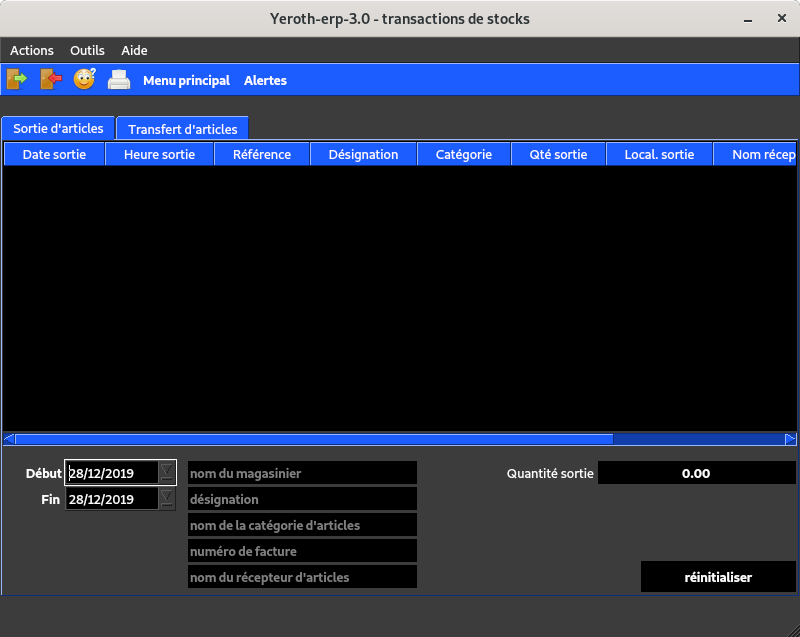
\includegraphics[scale=0.45]{images/yeren-transactions.png}
	\caption{La fen\^etre pour visualiser les sorties et les
		transferts d'articles.}
	\label{fig:yeren-transactions}
\end{figure}

La figure~\ref{fig:yeren-transactions} illustre
l'interface de \yeren pour visualiser les sorties et les
transferts d'articles.

Dans \yeren, une transaction est:
\begin{enumerate}[1)]
	\item une \textbf{sortie de stocks},
	\item ou bien un \textbf{transfert de stocks}.\\
\end{enumerate}

Une \textbf{sortie de stocks} est le retrait d'articles
par un client aupr\`es d'une boutique ou d'un d\'ep\^ot
de l'entreprise qui utilise \yeren.

Un \textbf{transfert de stocks} est un mouvement de stocks
d'une boutique ou d'un d\'ep\^ot de l'entreprise vers une
boutique ou d\'ep\^ot de votre entreprise.

%--------------------------------------------------------------

\nxsection{Voir les transactions sur une p\'eriode de temps}
\index{voir les transactions sur une p\'eriode de temps}

\begin{enumerate}[1)]
	\item S\'electionnez les dates de d\'ebut et de
	fin respectivement dans les champs de dates
	'D\'ebut' et 'Fin'.
\end{enumerate}

Les transferts de stocks s'affichent automatiquement
dans le $1^{\text{er}}$ premier onglet, pendant que
les sorties de stocks s'affichent automatiquement
dans le $2^{\text{\`eme}}$ onglet.	

L'utilisateur peut aussi ajouter les param\`etres suivants
\`a sa requ\^ete :

\begin{enumerate}[1)]
	\item le nom d'un magasinier (champs de texte 
	'\textbf{Magasinier}')
	\item la d\'esignation d'un l'article 
		(champs de texte '\textbf{D\'esignation}')
	\item la cat\'egorie d'un l'article 
		(champs de texte '\textbf{Cat\'egorie}')
	\item le num\'ero d'un bon de sortie 
		(champs de texte '\textbf{Num\'ero du bon de sortie}')
	\item le nom d'un r\'ecepteur
		(champs de texte '\textbf{Nom du r\'ecepteur}').
\end{enumerate}

Lorsque plus d'un param\`etre est utilis\'e pour
la requ\^ete, \yeren emploi l'op\'erateur logique
'\textbf{AND}' entre les diff\'erents param\`tres
pour g\'en\'erer le r\'esultat de la requ\^ete.

%--------------------------------------------------------------

\nxsection{Voir les transactions d'un magasinier}
\index{voir les transactions d'un magasinier}

\begin{enumerate}[1)]
	\item S\'electionnez dans le champs de texte
	'\textbf{Magasinier}' le nom du magasinier dont
	vous souhaitez observer les transactions effectu\'ees .
	
	\item Les transactions du magasinier choisi
	s'affichent automatiquement.
\end{enumerate}

%--------------------------------------------------------------

\nxsection{Voir les transactions d'un article}
\index{voir les transactions d'un article}

\begin{enumerate}[1)]
	\item S\'electionnez dans le champs de texte
	'\textbf{D\'esignation}' la d\'esignation de
	l'article dont vous souhaitez visualiser les
	transactions effectu\'ees .
	
	\item Les transactions de l'article choisi
	s'affichent	automatiquement.
\end{enumerate}

%--------------------------------------------------------------

\nxsection{Voir les transactions d'une cat\'egorie d'articles}
\index{voir les transactions d'une cat\'egorie d'articles}

\begin{enumerate}[1)]
	\item S\'electionnez dans le champs de texte
	'\textbf{Cat\'egorie}' le nom de la cat\'egorie
	d'articles dont	vous souhaitez visualiser
	les transactions effectu\'ees. 
	
	\item Les transactions de la cat\'egorie
	d'articles choisie s'affichent automatiquement.
\end{enumerate}

%--------------------------------------------------------------

\nxsection{Voir les transactions d'un bon de sortie}
\index{voir les transactions d'un bon de sortie}

\begin{enumerate}[1)]
	\item S\'electionnez dans le champs de texte
	'\textbf{Num\'ero du bon de sortie}' le num\'ero
	du bon de sortie dont vous souhaitez visualiser
	les transactions effectu\'ees.
	
	\item Les transactions du bon de sortie choisi
	 s'affichent automatiquement.
\end{enumerate}

%--------------------------------------------------------------

\nxsection{Voir les transactions d'un r\'ecepteur d'articles}
\index{voir les transactions d'un r\'ecepteur d'articles}

\begin{enumerate}[1)]
	\item S\'electionnez dans le champs de texte
	'\textbf{Nom du r\'ecepteur}' le nom de la
	personne dont vous souhaitez visualiser
	les transactions effectu\'ees, dont il a \'et\'e
	le r\'ecepteur.
	
	\item Les transactions de la personne choisi
	s'affichent automatiquement.
\end{enumerate}

%--------------------------------------------------------------

\nxsection{Imprimer le journal des transactions au format PDF}
\index{imprimer le journal des transactions au format PDF}

Il existe deux m\'ethodes pour imprimer 'le journal des
transactions' qui appara\^it dans la fen\^etre titr\'ee
'\textbf{Yeren - transactions}'.

\begin{itemize}[\mycheckmark{purplish}]
	\item \textcolor{purplish}{$\mathbf{1^{\text{\`ere}}}$ \textbf{m\'ethode}}\\
		Cliquez sur le lien
		'\textbf{Imprimer le journal des sorties/transferts}'
		qui se trouve dans le menu d\'eroulant '\textbf{Outils}'.\\

	\item \textcolor{purplish}{$\mathbf{2^{\text{\`eme}}}$ \textbf{m\'ethode}}\\
		Pressez simultan\'ement les boutons \bouton{CTRL}
		et \bouton{P} de votre clavier.
\end{itemize}

Un fichier au format PDF est alors g\'en\'er\'e et affich\'e.

\begin{figure}[!htbp]
	\centering
	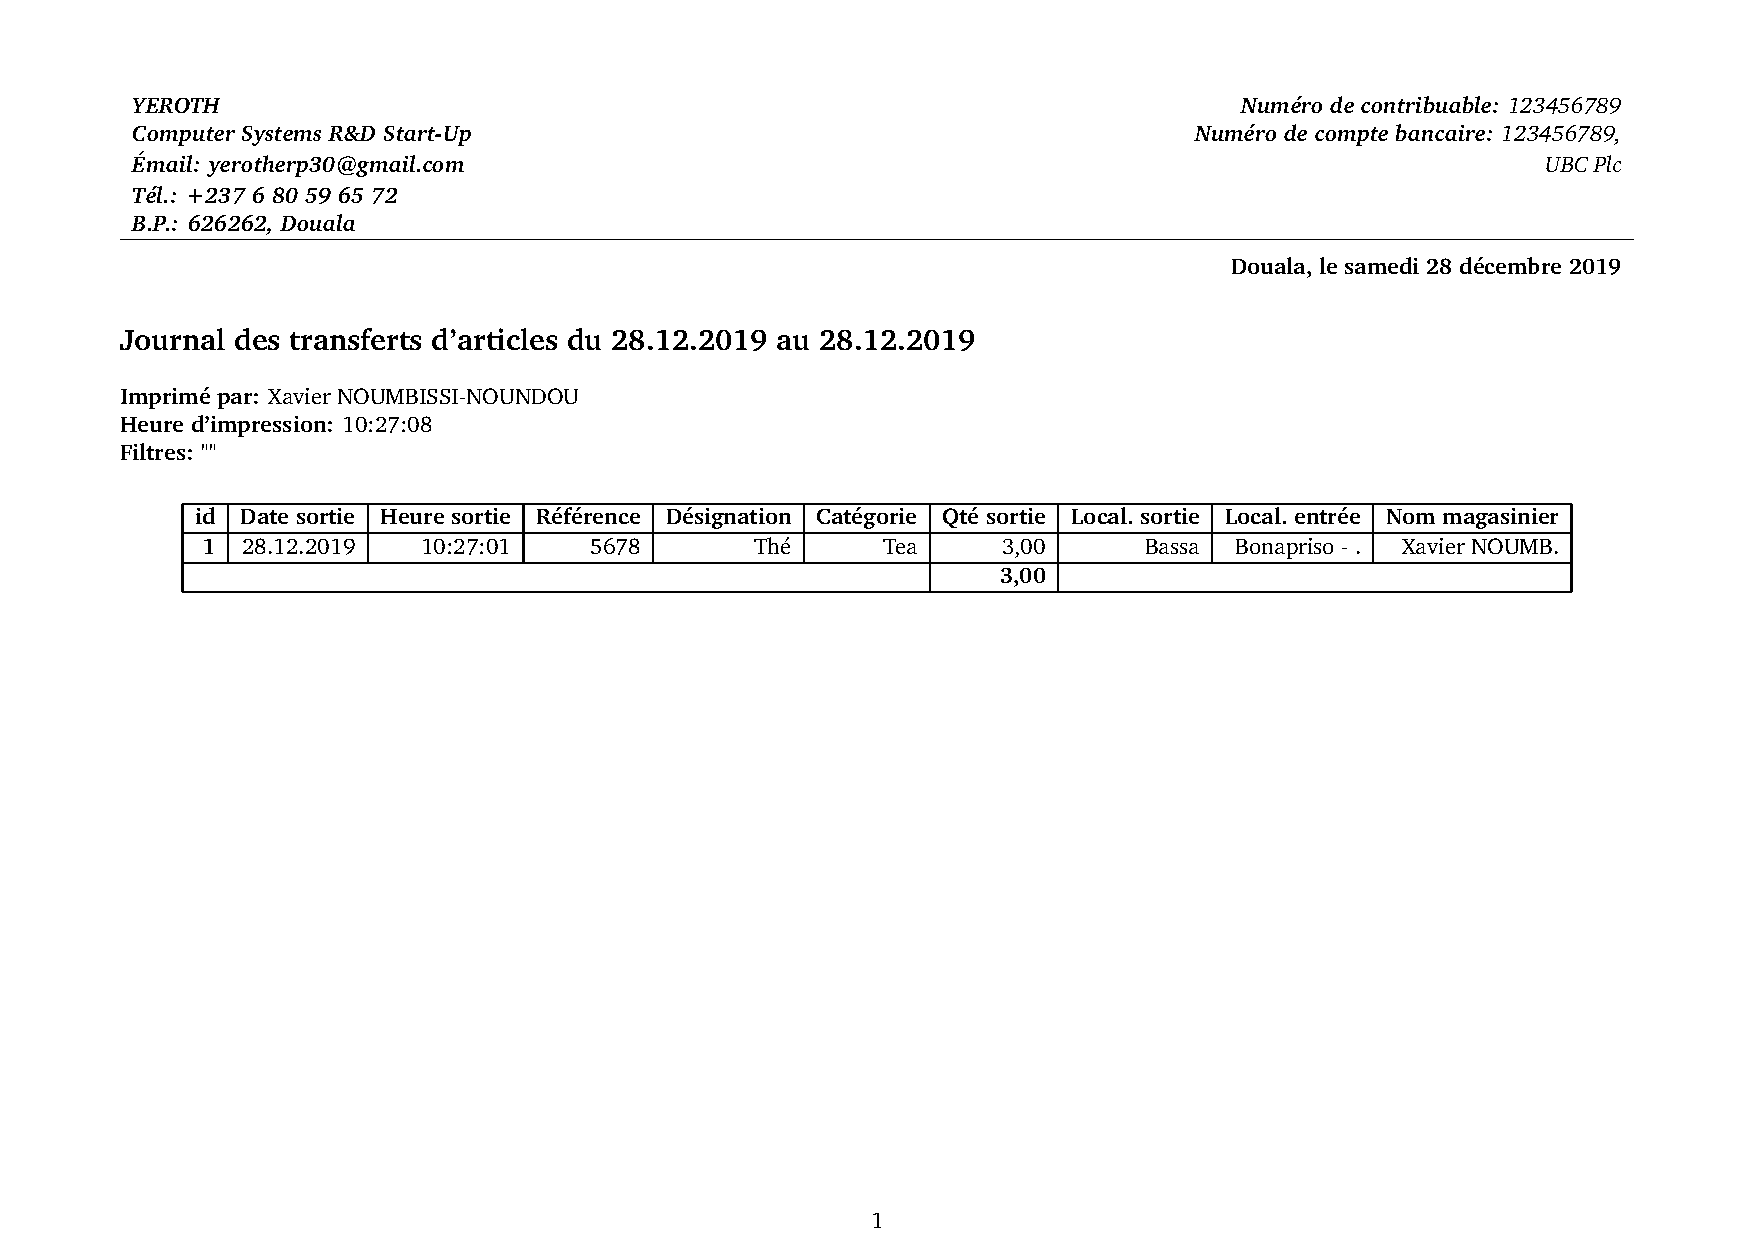
\includegraphics[scale=0.55]{images/yeren-journal-sortie-stocks-2017-06-14.pdf}
	\caption{Un journal de sorties des stocks.}
	\label{fig:yeren-journal-sorties-des-stocks}
\end{figure}

La figure~\ref{fig:yeren-journal-sorties-des-stocks} illustre un
exemple de journal de sorties des stocks au format PDF.

%--------------------------------------------------------------

\chapter{Les Informations G\'en\'erales}\label{chap:informations-generales}

\utilisateurs: \lienadmin, \liencaissier, \lienmagasinier, \lienmanager.\\

\chapintro{Ce chapitre d\'ecrit comment avoir acc\`es aux
informations publiques de l'entreprise et de \yeroth
(ex.: le si\`ege social de l'entreprise, la version
de \yeroth utilis\'ee, etc).}

\nxsection{Voir les d\'etails de l'utilisateur avec lequel
			on s'est enregistr\'e}
\index{voir les d\'etails de l'utilisateur avec lequel
		on s'est enregistr\'e}

\begin{figure}[!htbp]
	\centering
	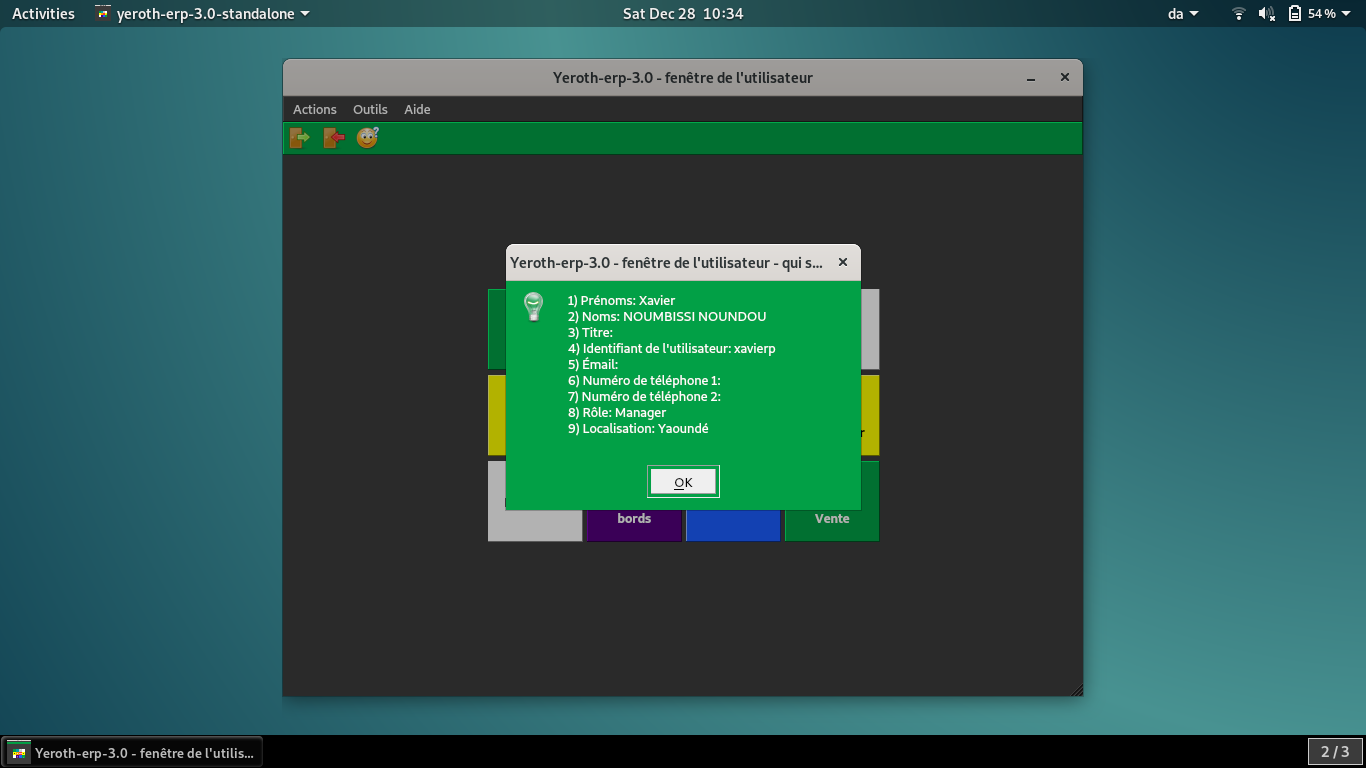
\includegraphics[scale=0.34]{images/yeren-qui-suis-je.png}
	\caption{Un example de la fonctionalit\'e 'Qui suis je ?'.}
	\label{fig:yeren-qui-suis-je}
\end{figure}

La figure~\ref{fig:yeren-qui-suis-je} illustre un example de
la fonctionalit\'e '\textbf{Qui suis je ?}'.

\`A partir de n'importe quelle fen\^etre de \yeroth, cliquez
sur le lien '\textbf{Qui suis je ?}' dans le menu d\'eroulant
'\textbf{Outils}' pour obtenir les informations suivantes
de l'utilisateur avec lequel on s'est enregistr\'e:

\begin{enumerate}[1)]
	\item l'\'email
	\item l'identification de l'utilisateur	
	\item la localisation
	\item les noms	
	\item le num\'ero de t\'el\'ephone 1
	\item le num\'ero de t\'el\'ephone 2	
	\item les pr\'enoms
	\item le r\^ole	
	\item le titre.
\end{enumerate}

%---------------------------------------------------------------

\nxsection{Voir les informations g\'en\'erales de l'entreprise}
\index{voir les informations g\'en\'erales de l'entreprise}

\`A partir de n'importe quelle fen\^etre de \yeroth (except\'e
les fen\^etres de l'administration), cliquez
sur le lien '\textbf{Informations sur l'entreprise}' dans
le menu d\'eroulant '\textbf{Aide}' pour obtenir les
informations suivantes de l'entreprise o\`u \yeroth
est ainsi d\'eploy\'e:

\begin{enumerate}[1)]
	\item l'\'email
	\item l'adresse
	\item la bo\^ite postale
	\item la d\'enomination de l'entreprise
	\item la localisation
	\item le num\'ero de contribuable	
	\item le pays
	\item les secteurs d'activit\'es
	\item le si\`ege social
	\item le t\'el\'ephone
	\item la ville.
\end{enumerate}

La figure~\ref{fig:yeren-informations-generales-entreprise}
illustre un example de la fonctionalit\'e 
'\textbf{Informations sur l'entreprise}'.\\

\begin{figure}[!htbp]
	\centering
	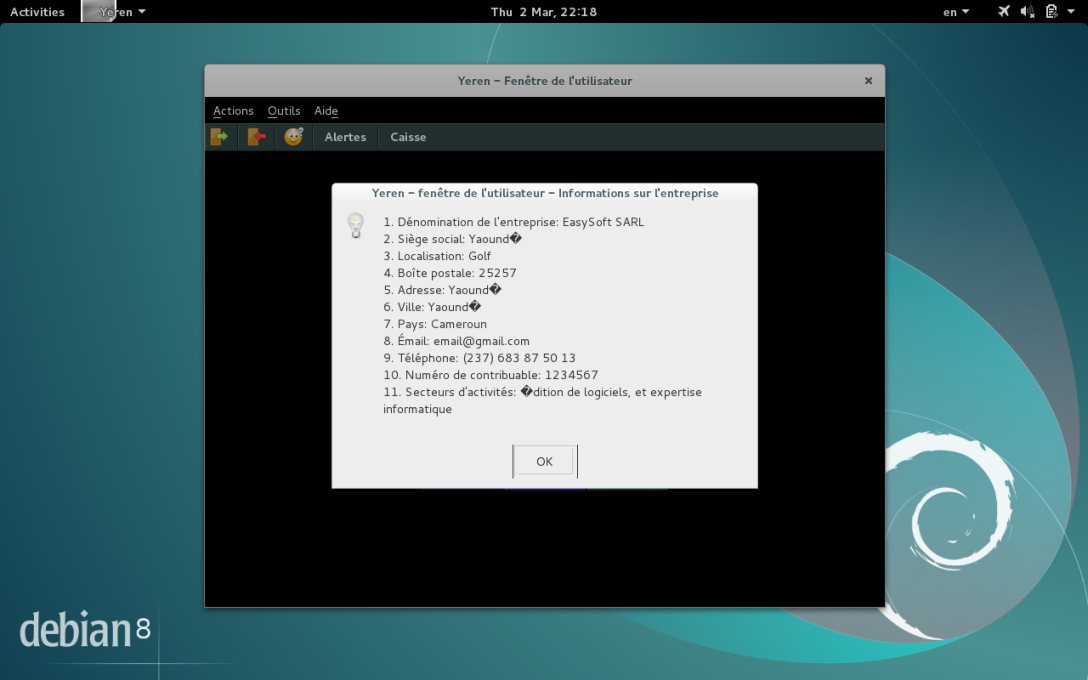
\includegraphics[scale=0.4]{images/yeren-informations-generales-entreprise.png}
	\caption{Un example de la fonctionalit\'e 'Informations sur l'entreprise'.}
	\label{fig:yeren-informations-generales-entreprise}
\end{figure}

%---------------------------------------------------------------

\newpage
\nxsection{Voir le manuel de l'utilisateur au format PDF}
\index{manuel de l'utilisateur au format PDF}

Il suffit de cliquer sur le lien '\textbf{Manuel de l'utilisateur (PDF)}'
qui se trouve dans le menu '\textbf{Aide}' de la fen\^etre
principale de chaque type d'utilisateur de \yeroth:

\begin{enumerate}[1)]
	\item \admin (voir figure~\ref{fig:fenetre-principale-admin})
	\item \caissier (voir figure~\ref{fig:fenetre-principale-caissier})
	\item \magasinier (voir figure~\ref{fig:yeren-fenetre-magasinier})
	\item \manager (voir figure~\ref{fig:yeren-fenetre-patron}).		
\end{enumerate}

%---------------------------------------------------------------

\nxsection{Voir la version de \yeroth que vous utilis\'e}
\index{voir la version de \yeroth que vous utilis\'e}

Il suffit de cliquer sur le lien '\textbf{\`A propos}' qui
se trouve dans le menu '\textbf{Aide}' de n'importe quelle
fen\^etre de \yeroth.

La figure~\ref{fig:yeren-apropos}
illustre un example de la fonctionalit\'e 
'\textbf{\`A propos}'.

\begin{figure}[!htbp]
	\centering
	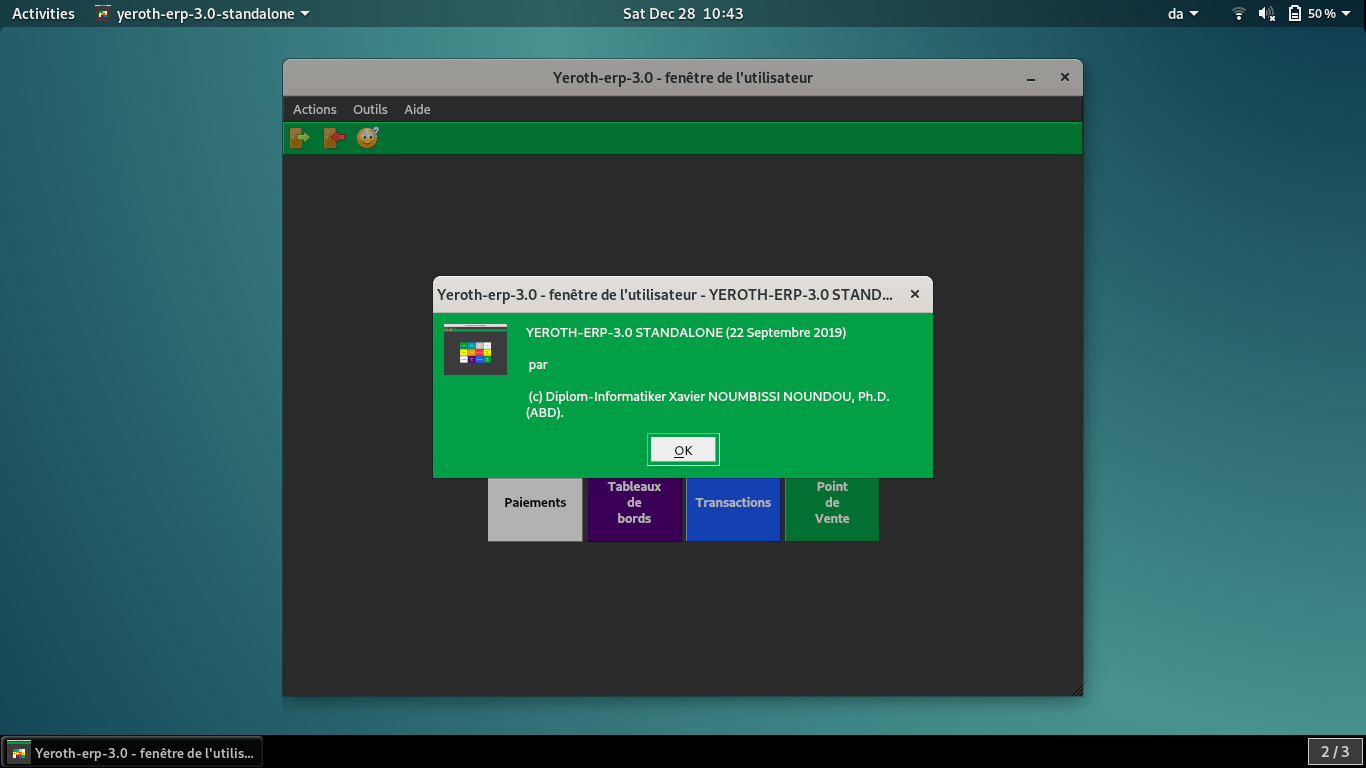
\includegraphics[scale=0.369]{images/yeren-apropos.png}
	\caption{Un example de la fonctionalit\'e '\`A propos'.}
	\label{fig:yeren-apropos}
\end{figure}



\chapter{Les Probl\`emes Connues et leurs Solutions}\label{chap:problemes-connues}
\index{probl\`emes connues ! solutions}
\index{probl\`emes connues et solutions}

\chapintro{Ce chapitre d\'ecrit quelques
probl\`emes qui peuvent survenir lors de
l'utilisation de \yeren et comment les r\'esoudre.}

\vspace{2cm}

\section{D\'emarrage du Syst\`eme d'Alerte}

Lorsque l'on d\'emarre le syst\`eme d'alerte,
le boutton \textbf{\textcolor{yerenColorGreen}{ON}}
n'est pas affich\'e aussit\^ot.

\chapter{Conclusion}

\yerotherpblack has a \thickclient
software--system architecture because we
found \thickclient software--system
architectures simpler than \webbrowserbased
software--system architectures.

A \webbrowserbased software--system
architecture has more drawbacks as
follows:

\begin{enumerate}[1)]
	\item it requires at least $3$ co--related 
		software--systems are required 
		(e.g.: DBMS, web server, application server.)
		to fully operate.
		
	\item A \webbrowserbased software--system
		requires at least $4$ layers within
		its logical system architecture
		(e.g.: client, presentation, logic, and data).

	\item A \webbrowserbased software--system
		potentially possesses more software
		security vulnerabilities because its
		implementation requires of the use of
		at least $2$ different programming 
		languages, and frameworks in combination.
\end{enumerate}

Table~\ref{tab:thickclient-application-againts-webbrowserbased-application}
demonstrates \thickclient software--system architecture
is better than \webbrowserbased software--systems.

\cleardoublepage
\phantomsection
\addcontentsline{toc}{chapter}{\textsc{Annexes}}
\appendix
\chapter{Les Raccourcis}\label{chap:raccourcis}
\index{les raccourcis}

\newcommand{\yerothraccouci}[1]{\textbf{\texttt{#1}}}

\chapintro{Ce chapitre pr\'esente les raccourcis
		   usuels de \yeren, sous forme de tableau,
		   pour acc\'eder \`a certaines fonctions.}


\begin{table}[!htbp]
\centering
\begin{tabular}{l|l}

Raccourcis									&
R\'esum\'e de la fonction					\\ \hline \hline

\yerothraccouci{Ctrl + H}					&
Appelle l'aide, r\'esum\'ee pour l'utilisateur	\\ \hline

\yerothraccouci{Ctrl + P}					&
Imprimer au format PDF						\\ \hline

\yerothraccouci{Ctrl + F}					&
Lancer l'interface de recherche				\\ \hline

\yerothraccouci{Ctrl + I}					&
R\'einitialiser la recherche				\\ \hline

\yerothraccouci{Ctrl + W}					&
Observer avec quel utilisateur
je me suis enregistr\'e (Qui suis je?)		
\end{tabular}
\caption{Tableau des raccourcis}
\label{tab:raccourcis}
\end{table}



% BACK MATTER
\backmatter
%\phantomsection
%\addcontentsline{toc}{chapter}{Bibliography}
%\bibliographystyle{alpha}
%\bibliography{yeren-pos-7-0-manuel-de-lutilisateur}

%\cleardoublepage
\phantomsection
\addcontentsline{toc}{chapter}{Index}
\printindex

\end{document}

